\cotefile{121}
\scanpage{1}

IMAG

INSTITUT MONTPELLIERAIN

ALEXANDER GROTHENDIECK

\figure{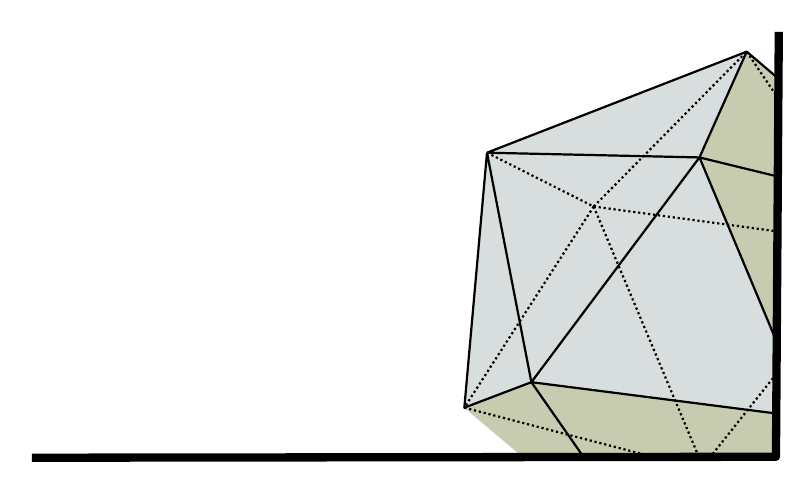
\begin{tikzpicture}[x=0.012cm,y=-0.012cm,line join=round]
\definecolor{facegray}{RGB}{216,222,222}
\definecolor{facegreen}{RGB}{199,204,176}
\path[fill=facegray] (495,139)--(770,32)--(803,60)--(800,458)--(529,458)--(471,409)--cycle;
\path[fill=facegreen] (770,32)--(720,144)--(800,335)--(802,164)--(803,60)--cycle;
\path[fill=facegreen] (471,409)--(542,382)--(800,415)--(799,458)--(529,458)--cycle;
\draw[thick] (495,139)--(770,32)--(803,60) (495,139)--(720,144)--(770,32) (495,139)--(542,382)--(471,409)--(495,139) (542,382)--(720,144)--(800,335) (720,144)--(802,164) (542,382)--(595,458) (542,382)--(800,415);
\draw[thick,densely dotted] (495,139)--(608,196)--(770,32) (608,196)--(800,222) (608,196)--(471,409) (608,196)--(718,458) (471,409)--(659,458) (770,32)--(803,81) (734,458)--(800,375);
\draw[line width=3pt] (13,462)--(801,461)--(804,11);
\end{tikzpicture}}

\scanpage{2}

Topologie

Modérée

\diagram{\begin{tikzcd}[column sep=small,row sep=small]
& \unsure{Z} \arrow[dl] & & \\
X \arrow[r] & \deleted{\unsure{I}} \arrow[u,hook] \arrow[d,hook] & I^{\unsure{n}} \arrow[ul,hook] \arrow[d] & I^{\unsure{n+1}} \arrow[l] \arrow[ddl] \\
& \unsure{Y} \arrow[r,hook] \arrow[d,hook] & X \arrow[d,hook] & \\
& I^{\unsure{n-1}} \arrow[r,hook] & I^{\unsure{n}} &
\end{tikzcd}}

\diagram{\begin{tikzcd}[column sep=small,row sep=small]
Y \arrow[d] & X \arrow[l,dash] \arrow[d] \\
\unsure{e} \arrow[r,hook] & I
\end{tikzcd}}

\diagram{\begin{tikzcd}[column sep=small,row sep=small]
I \arrow[r,dash] \arrow[d,dash] & I^2 \arrow[d,dash] \\
e \arrow[r,dash] & I
\end{tikzcd}}

\diagram{\begin{tikzcd}[column sep=small,row sep=small]
& & \displaystyle\coprod_{\alpha\in\unsure{Fl}\,I}X(\alpha) \arrow[d,shift left] \arrow[d,shift right] & \unsure{X_i\times_X X_j} \\
X_i \arrow[r,"\alpha"] \arrow[drr,"p_i"'] \arrow[ddr,dash] & X_j \arrow[dr,"\beta"] \arrow[dd,dash] & \displaystyle\coprod_{i\in\operatorname{Ob}I}X_i \arrow[d] & \displaystyle\coprod_{ij}X_i\times_X X_j \arrow[u,hook] \\
& & X \arrow[r,hook,"\beta"] \arrow[dl,"c"'] & M \\
& Z & &
\end{tikzcd}}

\margin{\begin{tabular}{|l}
a) $\beta\circ p_i$ \unsure{modéré} $\unsure{\forall i\in I}$.\\
b) $\beta$ injectif.\\[2ex]\hline
\end{tabular}}

\diagram{\begin{tikzcd}[column sep=small,row sep=small]
X\times_{Y'}X = X \arrow[r,"g"] \arrow[dr,"u"'] & Y' & Y \arrow[l,hook'] \\
& Z &
\end{tikzcd}}

\unsure{$q$}

\diagram{\begin{tikzcd}[column sep=small,row sep=small]
{}|X|\times_{|Y'|}|X| = |X| \arrow[r,"|g|"] \arrow[dr,"\deleted{\unsure{|u|}}"',"\mathrm{mod}"{description}] & {}|Y'| \arrow[d,"\unsure{v}","\mathrm{mod?}"'] & {}|Y| \arrow[l,hook'] \\
& {}|Z| &
\end{tikzcd}}

\diagram{\begin{tikzcd}[column sep=small,row sep=small]
R \arrow[r,shift left] \arrow[r,shift right] \arrow[d,equal] & X \arrow[r] & Y \\
X\times_Y X & & \\
X\times X \arrow[u,phantom,"\subset"{description}] \arrow[uur,shift left] \arrow[uur,shift right] & &
\end{tikzcd}}

\diagram{\begin{tikzcd}[column sep=small,row sep=small]
{}|X|\times|Z| \arrow[r,phantom,"\supset"{description}] \arrow[d,"{\unsure{\text{épi}}}"'{draw,circle,inner sep=1pt}] & \Gamma(\unsure{|u|}) \arrow[d,"\unsure{\mathrm{épi}}"] \\
{}|Y'|\times|Z| \arrow[r,phantom,"\supset"{description}] & \Gamma(\unsure{v})
\arrow[ul,phantom,"\mathrm{cont}"{description}]
\end{tikzcd}}

\diagram{\begin{tikzcd}[row sep=small]
(x,z) \arrow[d,dash] & z=\unsure{ux}\ (=vg(x)) \\
(gx,z) & z=\unsure{vg(x)}
\end{tikzcd}}

\mspage{1}

\scanpage{4}

\uline{(Structure modérée sur un espace)}

§ 1) $X$ ensemble \deleted{topologique}

$\deleted{\unsure{\mathcal E}}\inserted{F}$ ens. de parties de $X$, satisfaisant les conditions

b) $\deleted{\unsure{\mathcal E}}\inserted{F}$ stable pr réunions \unsure{finie|finies}

b') $\deleted{\unsure{\mathcal E}}\inserted{F}$ stable pr intersections finies

\unsure{a)} $F$ stable pr passage au complémentaire

\figure{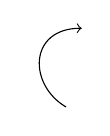
\begin{tikzpicture}[x=0.4cm,y=0.4cm]\draw[->] (0,0) .. controls (-1.2,0.7) and (-1.2,2.5) .. (0.5,2.5);\end{tikzpicture}}

Si $\deleted{\unsure{F}}\mathcal A_F$ est l'ens des fonctions sur $X$, à valeurs dans $\mathbb{Z}$ (disons), ne prenant qu'un nb fini de valeurs, et telles que $\forall n\in \mathbb{Z}$, on a $f^{-1}(\{n\})\in F$, \deleted{alors de sorte que} \inserted{alors} a) équivaut à la condition

\margin{\unsure{moyennant b)} $\mathcal A_F$ \unsure{contient l'ens des constantes}}

a') $\forall A\in F$, la fonction caractéristique $\varphi_A$ de $A$ est $\in\mathcal A_F$

et par suite \inserted{moyennant a)} la donnée de $F$ équivaut à celle de la partie $\mathcal A_F\subset \mathbb{Z}^X$. Ceci dit, \deleted{\unsure{les}} moyennant a) les conditions b) et b') sont équivalentes, et équivalent à la suivante :

b'') $\mathcal A_F$ est stable par produits finis

\deleted{\unsure{b''')} $\mathcal A_F$ est \unsure{\(\ne\varnothing\)} et stable pr \unsure{\(+\)}}

et alors $\mathcal A_F$ est \deleted{\unsure{aussi}} \inserted{même} stable pr sommes finies, et pr \unsure{l'inv. des signes} par $f\mapsto-f$, donc c'est un sous-anneau unitaire de $X^\mathbb{Z}$. Plus généralement, si $\Lambda$ est un anneau \deleted{\unsure{$\ne0$}} \inserted{non nul}, on peut remplacer dans tout ceci \inserted{$\mathbb{Z}$ par $\Lambda$, et} $\mathbb{Z}^X$ par $\unsure{K^X|\Lambda^X}$ : Moyennant a) et b) $\mathcal A_F$ est une sous-$\Lambda$-algèbre de $\deleted{\unsure{\mathcal A}}\Lambda^X$. Soit $\operatorname{Et}(X,\Lambda)$ l'alg. des fonctions ``\uline{étagées}'' sur $X$ à valeurs dans $\Lambda$ (i.e. ne prenant qu'un \deleted{\unsure{seul}} \inserted{nb fini de} valeurs). Alors $F$ est connu quand on connaît la sous-algèbre $\mathcal A_F$ de $\operatorname{Et}(X,\Lambda)$. Lorsque $\Lambda$ est intègre de corps

\mspage{5}

\scanpage{5}

de fractions $K$, on peut \unsure{prouver|penser} que les sous-algèbres $\mathcal A$ de $\operatorname{Et}(X,\Lambda)$ ainsi obtenues sont les traces sur $\operatorname{Et}(X,\Lambda)$ des sous-algèbres de $\operatorname{Et}(X,\Lambda)\otimes_\Lambda K\simeq\operatorname{Et}(X,K)$ [i.e. satisfaisant la condition que si $\varphi\in\operatorname{Et}(X,\Lambda)$ \deleted{est} et $\lambda\in\Lambda$ \deleted{$\unsure{\ne0}$} sont tels que $\lambda\ne0$ et $\lambda\varphi\in\mathcal A$, alors $\varphi\in\mathcal A$]

\figure{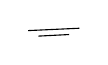
\begin{tikzpicture}[x=1cm,y=1cm]\draw (0,0)--(0.65,0.03);\draw (0.13,-0.07)--(0.52,-0.05);\end{tikzpicture}}

Nous supposons maintenant que $X$ est un espace topologique, et considérons la condition
\[
\text{c)}\quad\forall A\in F,\quad\text{on a}\quad\overline A\in F
\]
équivalente (moyennant a)) à
\[
\text{c')}\quad\forall A\in F,\quad\text{on a}\quad A^\circ\in F.
\]
Ceci implique donc que
\[
\dot A=\overline A-A^\circ\ \deleted{\text{est}}\ \in F
\]
donc la \inserted{\unsure{prem.}} partition de $X$ en $A^\circ$, $\unsure{(\complement A)^\circ}=X-\overline A$, $\dot A$ est formée d'éléments de $F$.

\deleted{d) $\forall A\in F$, \inserted{\deleted{\unsure{A}} tel que $A$ loc. fermé i.e. $\overline A-A$ fermé, (i.e. $A=B-C$ pour $B,C\in F$)} \deleted{$A$ est localement connexe, et les} \deleted{\unsure{les}} composantes connexes sont \inserted{ouvertes, de nb fini et} $\in F$.}

\mspage{6}

\scanpage{6}

Condition

d) $\forall A\in F$, \deleted{$A$ est dense} \inserted{\deleted{\unsure{l'intérieur|l'adhérence}} \inserted{l'intérieur} de $A$} dans $\overline A$ \inserted{est dense dans $\overline A$,} i.e. \deleted{$A$ est} \inserted{son complémentaire} \unsure{est d'intérieur} \deleted{\unsure{dans $\overline A$}} \uline{vide} dans $\overline A$ (et a fortiori dans $X$)

e) \deleted{\unsure{$A$}} $\forall$ suite décroissante $A_1\supset A_2\supset A_3\ldots$ de parties fermées \inserted{$(F)$} de $X$, où $\unsure{A_{n+1}}$ non dense dans $A_n$ pr tout $n$, on a $A_n=\varnothing$ pour $n$ assez grand.

\uline{NB} Si $\Phi$ est une partie de $\mathfrak P(X)$, alors la plus petite partie $F$ de $\mathfrak P(X)$ contenant $\Phi$ et satisfaisant a), b), est l'ens des \deleted{\unsure{les}} réunions finies d'ens de la forme $A\cap\complement B$, avec $A,B\in\Phi$. Ceci dit, prouvons

\uline{Prop} Si $F$ satisfait d et e, alors $F$ est ``engendré'' pr l'ens des parties fermées $\in F$.

Soit $F'\subset F$ l'ens engendré. \deleted{Soit $A\in F$, prouvons $A\in F'$.} Prouvons que tt $A\in F$ est $\in F'$. \deleted{Considérons $\dot A$} on a
\[
\overline A=A^\circ\cup bA\quad\text{d'où}\quad A=A^\circ\cup A\cap bA.\qquad A^\circ=\complement\overline{\complement A}\in F'
\]
grâce à \unsure{b)|a)} [$\to\overline{\complement A}\in F$ donc $\overline{\complement A}\in F'$), il reste à prouver que $A\cap bA\in F'$. Mais ceci nous \deleted{permet} ramène à prouver l'assertion analogue, en remplaçant $X$ par $bA=X_1$, $F$ \unsure{remplacé} par $F_1\subset\mathfrak P(X_1)$ ``\unsure{induit}'' pr $F$, \inserted{$A$ par $A_1=A\cap X_1$}. Or par d), $X_1$ est non dense dans $X$. On construit ainsi de proche \deleted{de} $X_0=X\supset X_1\supset X_2\supset\ldots\supset X_n\supset\ldots$, avec $X_{n+1}$ non dense dans $X_n$, et $A_n\in F_n=F|X_n$, tels que si $A_n\in F'_n\Rightarrow A\in F'$. Or $\exists n$ tel que $X_n=\varnothing$, \unsure{c.q.f.d.|ce qui}

\mspage{7}

\scanpage{7}

Soit $F_0$ un ens de parties fermées de l'espace topo $X$. Pour que l'ens $F\subset\mathfrak P(X)$ \inserted{satisfaisant a) b)} engendré pr $F_0$ soit tel que $F_0$ soit \inserted{exactement} l'ens des parties fermées $\in F$, il \unsure{faut|suffit} que $F_0$ soit stable pr intersections finies et réunions finies. Est-ce suffisant, i.e. est-il vrai alors que si une réunion finie
\[
A=\bigcup_i A_i\cap\complement B_i\qquad(A_i,B_i\in F_0)
\]
est fermée, alors $A\in F_0$ ? $\unsure{\Leftarrow}$

Or, $A=\overline A=\bigcup_i\unsure{\overline{A_i\cap\complement B_i}|A_i\cap\complement B_i}$, donc il suffit de savoir que, $\forall A,B\in F_0$, on a
\[
\overline{A\cap\complement B}\in F_0.
\]
\deleted{\unsure{et ceci est nécessaire et}} \deleted{\unsure{Réciproquement}} \inserted{Cette condition} \unsure{implique que} \unsure{si $F_0$ satisfait} \unsure{alors que $F$ satisfait c), et réciproquement,}

$\alpha)$ $F_0$ stable pr réunions finies

$\beta)$ — int. finies

$\gamma)$ $\forall A,B\in F_0$ alors $\overline{A\cap\complement B}\in F_0$

\deleted{Pour que} \inserted{Montrons} que $F$ satisfait \inserted{alors} d), \deleted{il faut que $F_0$ satisfasse $\delta)$ $\forall A,B\in F_0$ \deleted{\unsure{$A\cap B$}} l'intérieur de $A\cap\complement B$ dans}

En effet, si $\unsure{C}=\bigcup_i A_i\cap\complement B_i$, ($A_i,B_i\in F_0$), posons $C_i=A_i\cap\complement B_i$ \inserted{($C_i$ \unsure{loc\textsuperscript{t}} fermés)}, $D_i=\overline{C_i}\in F_0$ pr $\gamma)$, donc $C_i=D_i-E_i$ ($E_i=D_i-C_i$, fermé, \unsure{aussi} dans $F$, et $\in F_0$), alors, posant $D=\bigcup D_i$ \inserted{$=\overline C$}, $E_i$ est \deleted{non dense \unsure{dans $D_i$}} \inserted{a fortiori} non dense dans $D\supset D_i$, donc $E=\bigcup E_i$ est non dense dans $D$, donc
\[
D-E\subset C=\bigcup C_i\subset D
\]
\unsure{donc} $E$ fermé non dense $D$ donc l'int. rel. de $C$ dans $D=\overline C$ \deleted{est} \inserted{contient $D-E$, dense} \deleted{dans} dans $D=\overline C\ldots$

\mspage{8}

\scanpage{8}

Supposons donc que $F_0$ satisfasse $\alpha)$ $\beta)$ $\gamma)$, \deleted{et soit $A\in F$, on a $A=\bigcup_i C_i$ (finie) $C_i=D_i-E_i$, $E_i$ non dense}

Alors $\deleted{\forall A,B\in F_0}\inserted{\forall A\in F}$, $\deleted{\overline{A\cap\complement B}}\inserted{\overline A}$ est le plus petit \uuline{$\in F_0$} contenant $A\cap\complement B$ (donc est connu en termes de $F_0$ d'entrée, sans appel à la top. de $X$ !). Donc la \deleted{\unsure{Cond}} condition pour $A\subset B$, $A,B\in F$, que $A$ non dense $B$ i.e. $A'=B-A$ dense en $B$ i.e. $\deleted{\unsure{B}}B\subset\overline{A'}$, a un sens indépendamment de la connaissance de la top. de $X$. L'axiome e) sur $F$ peut donc s'expliciter en termes de $F_0$, \unsure{disons} :

$\delta)$ $\forall$ suite décroissante $A_1\supset A_2\supset\ldots\supset A_n\supset\ldots$ d'élts de $F$, tels que $\forall n$, $A_{n+1}$ \deleted{non} ``$F_0$-\unsure{rare}'' dans $A_n$ (i.e. \deleted{$A_n$ \unsure{soit} $\varnothing$} tout $\in F_0$ qui contient $A_n-A_{n+1}$ contient $A_n$), on a $A_n=\varnothing$ pour $n$ assez grand.

\uline{NB} On peut se demander, \unsure{indépendt} d'une topologie de $X$, pour un ensemble $F_0$ de parties de $X$, quand il existe une top. sur $X$ pour laquelle $F_0$ \unsure{satisfais|satisfait} : $\alpha)$ $\beta)$ $\gamma)$ (et éventuellement $\delta)$). Il faut et s. que $F_0$ satisfasse $\alpha)$ $\beta)$ (qui ne font pas appel à une topologie de $X$), et :

\mspage{9}

\scanpage{9}

$\gamma')$ $\forall A,B\in F_0$, l'intersection des $\in F_0$ qui contiennent $A\cap\complement B$ est $\in F_0$ (i.e. il y a un plus petit $C\in F_0$ qui contienne $A\cap\complement B$).

C'est suffisant, car on prend la top. $T$ \deleted{\unsure{formée par}}\inserted{dont les fermés sont} les intersections quelconques d'élts de $F_0$ [ils sont stables par réunions finies, comme on voit tout de suite]. Cette topologie \inserted{est} \deleted{satisfait} visiblement la moins fine parmi celles qu'on envisage. Elle est caractérisée par le fait qu'elle satisfait la condition

\deleted{\unsure{l'ensemble ouvert}} $(*)$ Tout ouvert de $X$ est réunion d'ouverts de $X$ qui sont $\in F$, ou encore tout fermé de $X$ est int. de fermés qui sont $\in F$, ou encore $\deleted{\forall}\unsure{\forall}$ les $x\in X$ a un syst. fond. de voisinages $\in F$ (ou de voisinages ouverts $\in F$) ....

\margin{\deleted{\uline{Condition f} Si $A\in F$ est loc. fermé (donc de la forme $B-C$, $B,C\in F_0$, $C$ non dense $B$) alors \deleted{\unsure{l'ens des}} composantes connexes de $A$ \deleted{\unsure{est}} \inserted{\unsure{sont en nb}} \uuline{\unsure{finies|fini}} (donc \deleted{\unsure{fermées}}\inserted{\unsure{ouvertes}}) et sont $\in F_0$.}}

\uline{NB} Supposons que $F$ satisfasse a)b)c)d), \unsure{je dis que|pr dire que} \deleted{\illegible{2}} si $A\in F$, alors $\dot A$ \inserted{\figure{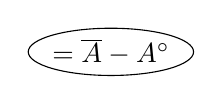
\begin{tikzpicture}[baseline=-0.6ex]\draw (0,0) ellipse (1.05 and .3);\node at (0,0) {$=\overline A-A^\circ$};\end{tikzpicture}}} est \uline{rare} dans $X$, \deleted{En effet, $\dot A=\overline A-A^\circ$, et $A^\circ$, i.e. $\dot A$} l'intérieur \inserted{$U$} de $\dot A$ est vide. On sait que $U\in F$, \unsure{nous restreignons nous à} $U$ [cela conserve a)b)c)d)] on est ramené à prouver que si $\overline A=X$, $A^\circ=\varnothing$, alors $\deleted{\unsure{X|A}}=\varnothing$. \inserted{\unsure{on utilise par d)} $A^\circ$ \unsure{est} dense dans $\deleted{X}=\overline A$ ...}

\mspage{10}

\scanpage{10}

\uline{Condition f)} $\forall A\in F$, $A$ loc. fermé (i.e. $A=B-C$, $B,C\in F_0$) les comp. connexes de $A$ sont en nb fini (donc ouvertes dans $A$) et $\in F$.

\figure{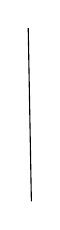
\begin{tikzpicture}\draw (0,2.2)--(.04,0);\end{tikzpicture}}

Cela implique donc que $A$ \inserted{loc. fermé, $\in F$} est connexe \unsure{ssi} \deleted{que} $\deleted{\unsure{B}}A',A''\in F$, $A'\cap A''=\varnothing$, $A'\cup A''=A$, $A'$ et $A''$ fermés ds $A$ (trace donc sur $A$ d'éléments de $F_0$), on a $A'=\varnothing$ ou $A''=\varnothing$ : c'est donc là une condition qui ne fait pas intervenir la top. de $X$, mais $F_0$ directement. De plus, \deleted{\unsure{on a} $(\varphi)$ si $A$ est loc. fermé}\inserted{$F_0$ satisfait} $(\varphi)$ $A=B-C$, avec $B,C\in F_0$, $C\subset B$, alors $A$ se décompose en réunion disjointe \uuline{finie} \unsure{d'éléments|d'élts} de $F$ \unsure{rel. ferm|rel. fermés} dans $A$ \inserted{(i.e. traces sur $A$ d'$\in$ de $F_0$)}, qui sont ainsi $F_0$-connexes. \deleted{C'est là une condition \inserted{\unsure{portant}} sur $F_0$).}

Si les ouverts $\in F$ forment une base de la top. de $X$, alors la condition f) (qui peut être considérée comme une condition sur l'ens de parties $F_0$) implique que les $A\in F$ (du moins ceux qui sont loc. fermés --- en fait cette restriction est inutile) sont \uline{loc. connexes}.

\mspage{11}

\scanpage{11}

\uline{\S\ 2) (Décompositions cellulaires)} \deleted{\unsure{\S\ 1}}

Soit $\mathcal P=(X_i)_{i\in I}$ une partition \inserted{finie} de $X$, et soit $F_{\mathcal P}$ l'ens des parties de $X$ qui sont des réunions \deleted{finies} de $X_i$. Alors \deleted{\unsure{le}} $F_{\mathcal P}$ satisfait les conditions a), b), et $\mathcal A_{(F_{\mathcal P})}$ est l'algèbre des fonctions sur $X$ à valeurs dans $\Lambda$ qui sont constantes sur chaque $X_i$; i.e. qui se factorisent par l'ens quotient $X/R$, où $R$ \deleted{\unsure{la}} est la relation d'équivalence associée à la partition.

\margin{$F_{\mathcal P}$ est en \unsure{corres.} biunivoque avec l'ens des parties de $X/R$.}

\margin{\uline{NB} La partition $\mathcal P$ est connue quand on connaît $F_{\mathcal P}$ \deleted{\unsure{la}} : elle est formée des \unsure{éléments|élémts} $\ne\varnothing$ minimaux de $F_{\mathcal P}$. Les $\mathcal P$ \unsure{correspondent aux} $F$ \uuline{finis}.}

Supposons $X$ un espace topologique. Alors la condition c) équivaut à la suivante : \textcircled{$1^\circ$} $\forall i\in I$, $\overline X_i$ est une réunion des $X_j$ (i.e. est saturée par $R$). \deleted{Montrons} \deleted{\unsure{modération}.} \inserted{La condition d) équivaut à}

\deleted{que cela implique que \textcircled{$2^\circ$} chaque $X_i$ est \uline{loc. fermé} \inserted{dans $X$}, i.e. ouvert dans $\overline X_i$, ou encore que $\overline X_i-X_i$ est fermé. En effet, c'est une réunion des ``feuilles'' $X_j$, avec $j\ne i$, or si (pour \inserted{un} $j\ne i$) ... $X_j\subset\overline X_i$, je dis que l'on a $\overline X_j\cap X_i=\varnothing$ : en effet, je dis que ceci équivaut à :}

\margin{Mais $1^\circ$ + les $X_i$ loc. fermés n'implique \unsure{pas} \deleted{\unsure{ceci}} (\unsure{Ex} : \deleted{\unsure{le}} $X=\{x\}\unsure{\amalg|\cup}(X-\{x\})$, $x$ pt fermé non isolé) \deleted{\unsure{de $X$ et leurs complémentaires $\in F$ (pt. fermé isolé)} $X$ étant séparé}.}

$2^\circ)$ Si $i,j\in I$, alors $\overline X_i=\overline X_j\Longrightarrow X_i=X_j$.

\deleted{\unsure{Néc}.} \uline{Néc} \deleted{\unsure{évident}} \inserted{Comme \unsure{e)|c)} est vérifié trivialement, \unsure{chaque} $X_i$ est \unsure{réunion finie de} parties \unsure{étrangères|étagées} loc. fermées, donc \unsure{l’un au moins est|son intérieur est} $\ne\varnothing$ \unsure{dans} $\overline X_i$.}

\deleted{Si $\overline X_i=\overline X_j\ (=Z)$, comme $X_i$ et $X_j$ sont \unsure{denses} dans $Z$, \unsure{donc} $\unsure{Z}$, \unsure{d'où} $X_i\cap X_j\unsure{\ne}\varnothing$, \unsure{vide}.}

\inserted{\unsure{et} $\unsure{X_j^\circ}$ \unsure{est loc. fermé, donc dense dans} $\overline X_i$. Mais alors $\overline X_i=\overline X_j\Longrightarrow X_i\cap X_j\ne\varnothing$, donc $i=j$, OK.}

Je dis que $1^\circ)$ et $2^\circ)$ impliquent que les $X_i$ sont \uline{loc$^t$ fermés}. En effet,

\mspage{12}

\scanpage{12}

Considérons la relation dans $I$
\[
i\unsure{<|\le}j\overset{\mathrm{déf}}{\Longleftrightarrow}\overline X_i\subset\overline X_j
\]
(Relation d'incidence des feuilles). C'est une relation de préordre, et grâce à 2) une relation d'ordre. Soit $\deleted{X_i}\inserted{X_{i_0}}$ une feuille minimale. Alors, comme $\overline X_{i_0}$ donc $\overline X_{i_0}-X_{i_0}$ est une réunion de feuilles, on voit que $\overline X_{i_0}\unsure{-}X_{i_0}=\varnothing$ à cause de la condition minimale : Une feuille minimale (pour la relation d'incidence) est fermée. Ceci étant, on raisonne par récurrence sur le nb des feuilles, en remplaçant $X$ par $X-X_{i_0}$ et la partition induite $(X_i)_{i\in I-\{i_0\}}$.

\margin{\uline{NB} Si $X_i$ n'est pas \uline{incidente} à $X_j$ alors $X_i\cap\overline X_j=\varnothing$, \deleted{donc} $\overline X_j\cap\overline X_i$ \uline{rare} dans $\overline X_i$.}

\inserted{Il est clair maintenant que $F_{\mathcal P}$ est engendré par ses parties fermées $F_0$, donc d) est satisfait automatiquement !}

\deleted{\unsure{Partition cellulaire de}} \inserted{\uline{Décomposition cellulaire}} (finie) de $X$ : satisfaisant $1^\circ)$ et $2^\circ)$.

Elle est ``\uline{stricte}'' si elle satisfait de plus

3) Les $X_i$ sont \deleted{\unsure{localement}}\inserted{connexes}.

Je dis que [moyennant $1^\circ)$ et $2^\circ)$] 3) équivaut à la condition f) pour $F_{\mathcal P}$, i.e. que $\unsure{\forall}$ $A\in F_{\mathcal P}$ qui est loc fermé est \deleted{\unsure{localement connexe|réunion loc connexe}} \inserted{a} des comp. connexes $\in F_{\mathcal P}$ \inserted{et en nb fini} \deleted{\uline{\unsure{C'est suffisant}}}. En effet,

$d)\Longrightarrow3)$, car $X_i$ étant loc$^t$ fermé et $\in F_{\mathcal P}$, \deleted{\unsure{alors}}

\mspage{13}

\scanpage{13}

\deleted{étant loc. connexe, et} ses composantes connexes \unsure{sont} $\in F_{\mathcal P}$ --- or $X_i$ étant un élément $\ne\varnothing$ minimal de $F_{\mathcal P}$, il s'ensuit que $X_i$ est connexe. Inversement, $3)\Longrightarrow d)$.

Soit en effet $A\in F_{\mathcal P}$ [loc fermé] \inserted{\unsure{pas néc}}. Quitte à remplacer $X$ par $A$, et la partition de $X$ par la partition induite [qui satisfait encore 1), 2), 3)] --- \deleted{\unsure{ceci}} c'est trivial sauf pour $2^\circ$, \inserted{mais} \deleted{\unsure{c'est vrai encore car $A$ est ouvert, mais}} si $X_i,X_j\subset A$, $i\ne j$, et $\overline X_i\deleted{\unsure{\cap}}\cap A=\overline X_j\cap A$, \deleted{comme \unsure{on a} $X_i$}\inserted{comme $X_i\subset\overline X_i\cap A$ et $X_j\subset\overline X_j\cap A$}, on aura $X_i\subset\overline X_j$ et $X_j\subset\overline X_i$ donc $\overline X_i=\overline X_j$ donc $X_i=\uline{X_j}$)

On est ramené à prouver \deleted{que $X$ est loc. connexe et} que les composantes connexes \deleted{\unsure{ouvertes}} de $X$ sont \deleted{\unsure{ouvertes et}} réunions de feuilles. Or les $X_i$ étant connexes, \deleted{les $\overline X_i$ aussi. Donc} \deleted{\unsure{et réunion des} $X_j$} les composantes connexes \inserted{de $X$} sont \inserted{bien} des réunions d'\unsure{ens} $\unsure{\overset{\deleted{-}}{X_i}|X_i}$, \deleted{\unsure{donc} (grâce à $2^\circ$) \unsure{disjoints} et \unsure{réunion des} \illegible{2}} Donc il n'y en a qu'un nb fini, \deleted{donc les composantes connexes sont \deleted{\unsure{f}} ouvertes, constituent une partition finie de $X$ \deleted{par des} par des fermés.}

Soit $Y=X/R\ (\simeq I)$ l'espace quotient. C'est un espace \uline{top} \uline{fini}. \deleted{\unsure{On a} $\unsure{\overline{\{i\}}}$} Si $i\in I$, $\unsure{\{i\}|\overline{\{i\}}}$ le plus petit

\mspage{14}

\scanpage{14}

ens fermé de $I$ contenant $i$) \deleted{à l'image}\inserted{correspond} au plus petit ens. fermé \uline{saturé} de $X$ contenant $X_i$, c'est donc $\overline X_i$ par 1). Donc $j\in\overline{\{i\}}$ ssi $X_j\subset\overline X_i$ i.e. $\overline X_j\subset\overline X_i$ : la relation d'incidence est la relation de spécialisation. La condition \inserted{$2^\circ)$ : $\overline X_i=\overline X_j\Longrightarrow X_i=X_j$} i.e. $i=j$ \uline{signifie} donc que $I$ est ``présobre'' \deleted{\unsure{condition}} i.e. $\overline{\{i\}}=\overline{\{j\}}\Longrightarrow i=j$. Si $\varphi:X\to I$ est l'application de passage au quotient, la condition $1^\circ)$ \uline{signifie} que $J\mapsto\varphi^{-1}(J)$ commute à l'adhérence (ou encore, à l'intérieur) i.e. que $\varphi$ est une application \uline{ouverte}.

Ainsi, on voit que les décompositions cellulaires \inserted{(finies)} de $X$ correspondent aux \deleted{\unsure{esp}} espaces quotients \inserted{finis} de $X$ qui sont présobres, et tels que $X\to X/R$ soit \uline{ouverte}.

\S\ 3 \deleted{\unsure{Théorème|Admissibilité}} \inserted{\uline{Décompositions cellulaires \unsure{Fin-admiss.|$F$-admiss.} : th. d'existence}}

Si $F$ est comme \unsure{ds|dans} \S\ 1, une décomposition cellulaire de $X$ est dite $F$-admissible (ou partition $F$-admissible) si ses feuilles sont $\in F$, i.e. si $F_{\mathcal P}\subset F$.

\mspage{15}

\scanpage{15}

\margin{\deleted{\unsure{On le fait} (\unsure{fini}) \unsure{plus bas pour} $F$}}

\uline{Prop.} \deleted{(\unsure{1})} Soit $F\subset\mathfrak P(X)$ satisfaisant les conditions a) b) c) \inserted{d) e)} du \S\ 1, et soit $\Phi\subset F$ une partie finie de $F$. Alors il existe une décomposition cellulaire $F$-admissible de $X$, telle que les $Y\in\Phi$ sont des réunions de feuilles. Parmi \unsure{ttes ces|les ces} décompositions cellulaires, il y en a une plus \deleted{fine} grossière \deleted{que les autres}\inserted{(qui est donc \unsure{uniqt déterminée|unique déterminée})}.

\deleted{\unsure{Supp} $\Phi$ \unsure{stable par} $\unsure{f_0|b}$} Soit
\[
\unsure{X'|Z'}=\bigcup_{Y\in\Phi}\dot Y,
\]
c'est une réunion finie de parties fermées rares de $X$, donc est une partie \uline{rare} de $X$, soit $\deleted{\unsure{X'=X_2}}$ $U=\deleted{\unsure{X}}\complement X'$. Les traces \inserted{$Y\cap U$} sur $U$ des $Y\in\Phi$ sont des \deleted{ouverts} parties à la fois ouvertes et fermées \deleted{donc sont} en \uline{nb fini}. Il y a donc (lemme \inserted{ensembliste} immédiat) dans $U$ une plus \deleted{fine}\inserted{grossière} partition \inserted{(finie)} par des $U_i$ \deleted{ouverts} telles que les $Y\cap U$ soient des réunions \inserted{(finies)} de $U_i$; de plus, chaque $U_i$ est une intersection \inserted{(finie)} des tels ensembles $Y\cap U$, \inserted{donc est aussi ouvert et fermé.} Ceci étant, si la prop. est prouvée pour \deleted{\unsure{les}} $(X,\Phi)$ remplacé par
\[
\left(X',\Phi'=\{Y\cap X'\mid Y\in\Phi\}\inserted{\cup\{\overline U_i\cap X'\}_{i\in\unsure{I}}}\right),
\]

\mspage{16}

\scanpage{16}
il est immédiat qu'il l'est pour $(X,\Phi)$: si $(X'_j)_{j\in J}$ est la partition cherchée de $X'$, celle de $X$ est formée des $X'_j$ et des $U_i$. Ceci nous fournit un principe de dém. récurrente, si on suppose que $F$ satisfait la condition e)

\deleted{(Dim) Toute suite \inserted{\unsure{finie}} \deleted{décroissante}\inserted{$X_1\supset X_2\supset\cdots\supset X_n$} de parties fermées $\in F$ de $X$, telles que $\forall i$, $X_{i+1}$ soit non dense $X_i$, on a $X_n=\varnothing$ pour $n$ assez grand.}
\margin{\unsure{résulte en particulier de l'existence d'une dimension \unsure{finie}}}

\uline{Cor 1} Si $F$, \deleted{en plus des conditions}\inserted{satisfait les} a) b) c) \inserted{d) e)}\deleted{, satisfait la condition (Dim)}, alors $F$ est réunion filtrante des sous-ens. \inserted{de la forme} $F_{\mathcal P}$ (associés aux décompositions cellulaires \deleted{\unsure{compatibles}} $F$-admissibles de $X$).

\uline{Cor. 2} L'ens \inserted{$\unsure{\mathcal E|\mathcal D}$} des décompositions cellulaires $F$-admissibles, pour la relation d'ordre du raffinement, admet des bornes sup. pour les \inserted{sous} ens. finis de \deleted{\unsure{même}}\inserted{$\unsure{\mathcal E|\mathcal D}$}.
\mspage{17}

\scanpage{17}
\uline{Remarque} Supposons que $F$, en plus de a) b) c) \deleted{(et (Dim))}\inserted{d) e)} satisfasse encore f). Alors il existe une décomposition cellulaire \uline{stricte} \inserted{$\mathcal P$} (i.e.: feuilles connexes) $F$-admissible telle que les $Y\in\Phi$ soient des \inserted{réunions} feuilles, et \unsure{$=$|---} parmi ces $\mathcal P$, il y en a une plus grossière. La dém. est la \unsure{même}, mais au lieu de prendre les $U_i$ précédents, on prend leurs composantes connexes.

Donc $F$ est réunion filtrante de $F_{\mathcal P}$ avec les $\mathcal P$ décompositions cellulaires à \uline{feuilles connexes}; et ces décompositions cellulaires admettent des sup. finis.

\uline{§ 4} \inserted{(Décompositions cellulaires $F$-modérées \uline{régulières})}
Supposons maintenant donné une partie $F_r$ de $F$ \deleted{\unsure{les|elle}} formée d'éléments de $F$ \deleted{\unsure{tous}}\inserted{loc.} fermés: ce seront les parties $F$-\uline{régulières} de $F$. On suppose que

\textcircled{$\unsure{B|S}$} Pour tout $Y\in F$, $Y$ \deleted{\unsure{loc.}} fermé, parmi les parties \inserted{rel.} ouvertes $U$ de $Y$ qui sont $\in F_r$, il y en a une plus grande $Y_{\mathrm{reg}}$, et \deleted{\unsure{Y}} celle-ci est dense dans $Y$ i.e. son complémentaire $Y-Y_{\mathrm{reg}}=Y_{\mathrm{sing}}$ est rare en $Y$.
\mspage{18}

\scanpage{18}
Ceci dit, une décomposition cellulaire $\mathcal P$ de $X$ est dite $F$-\uline{régulière} si \deleted{les feuilles sont $\unsure{\in F_r}$}\inserted{$F_{\mathcal P}$ muni de la notion de \uline{régularité} induite par $F,F_r$ satisfait la condition $\unsure{S|B}$, i.e. \deleted{$\unsure{\mathcal P}$} \unsure{plus précisément} $\forall\deleted{\unsure{X}}Y$ fermé $\mathcal P$-saturé $Y_s$ est $\mathcal P$-saturé. (\uline{Ceci implique que les feuilles sont} $\in F_r$)}

\uline{Prop.} Sous les conditions a) b) c) d) \unsure{e)} \deleted{\unsure{f)}} sur $F$, et la condition $(\unsure{S|B})$ sur $F_r\subset F$, si $\Phi\subset F$ est une partie finie, il existe une partition $F$-\uline{régulière} de $X$, et \unsure{$=$|---} une plus \uline{grossière} telle partition. Si $F$ satisfait \unsure{$=$|---} f), alors il existe une partition $F$-\uline{régulière} de $X$ à feuilles connexes, et une plus \uline{grossière} telle.
\figure{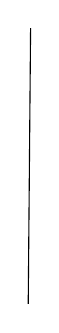
\begin{tikzpicture}[x=1cm,y=1cm]\draw (0,0)--(0.03,3.5);\end{tikzpicture}}

\inserted{QPS $\Phi$ stable par $\unsure{\complement}$ .}
Soit
\[
X'=\bigcup_{Y\in\Phi}\dot Y\cup\mathring Y_{\mathrm{sing}},\qquad U=X-X'.
\]
Les $Y\cap U$ sont ouverts et fermés, et \uline{réguliers}. On continue comme plus haut, \inserted{avec les $U_i$, mais dans $\Phi'$ on met aussi les $(\overline{U_i})_{\mathrm{sing}}$} Dans le cas où $F$ satisfait d), on passe encore \inserted{avant} aux composantes connexes des $U_i$.

\inserted{\uline{Cor. 1}} Donc $F$ est réunion filtrante de $F_{\mathcal P}$ où $\mathcal P$ est à feuilles $F$-\uline{régulières} (resp. $F$-\uline{régulières} et connexes, si $F$ satisfait d)).

\uline{Cor 2} Sup \inserted{finis} dans les partitions $F$-\uline{régulières} (resp. à fibres connexes)

\uline{Cor 3} Partition $F$-régulière canonique de $X$
\mspage{19}

\scanpage{19}
\deleted{\uline{§ \unsure{4|5} \unsure{Décompositions régulières}}}

\uline{§ 5} \uline{Localisation}

Soit $F$ satisfaisant a) b) c) d) e), ou encore $F_0$ satisfaisant $\alpha\,\beta\,\gamma\,\delta$ (c'est kif kif). Soit $A\in F$, considérons
\[
F_A=\{B\in\mathfrak P(A)\mid B\in F\}.
\]
Evidemment $F_A$ satisfait a) b) c), satisfait-il aussi d) et e)? Pour d), \unsure{cela|ceci} provient du fait immédiat que $F_A$ est engendré par $(F_A)_0$ i.e. que $\unsure{\forall A|U_A}\in F_A$ est réunion finie de parties loc fermées \inserted{$\in F_A$} de $A$. \deleted{\unsure{E}} Enfin, pour e) on considère
\[
A\supset A_1\supset A_2\supset\cdots\supset A_n\supset\cdots
\]
$A_i\in \unsure{F_A|F_{\deleted{A}}}$, $A_i$ rel. fermé dans $A$, $A_{i+1}$ rare dans $A_i$.
\margin{On peut partir d'une partie \uline{quelconque} $A$ de $X$, et poser $F_A=\{B\cap A\mid B\in F\}$; alors $F_A$ satisfait a) b) c) d) e)}

Alors $\overline{A_i}$ rare dans $\unsure{\overline{A_{i-1}}|\overline{A_i}}$, \deleted{\unsure{donc nulle pour $i$ grand on a}} (car $A_{i\deleted{\unsure{+1}}}-A_{i+1}$ dense dans $A_i$ dense dans $\overline{A_i}$, \deleted{donc $A_{i+1}$} \unsure{or|$\cap$}
\[
A_i-A_{i+1}=A_i-\underbrace{\overline{A_{i+1}}\cap A_i}_{A_{i+1}}\subset\overline{A_i}-\overline{A_{i+1}}
\]
qui est donc dense dans $\overline{A_i}$) donc pour $i$ grand on a $\overline{A_i}=\varnothing$ donc $A_i=\varnothing$ cqfd.

Prouvons que si $F$ satisfait aussi f), il en est de \unsure{$=$|même} de $F_A$. C'est trivial si $A$ loc fermé. Il reste à prouver que si $A\in F$ quelconque, ses comp. conn. sont $\in F$ et en nb fini. Or $A=\bigcup Z_i$, les $Z_i$ loc fermés, et par f) QPS les $Z_i$ \uline{connexes}. Donc les composantes
\mspage{20}

\scanpage{20}
connexes de $A$ sont réunions de $Z_i$, donc en nb fini et $\in F$.

Nous supposons maintenant que les ouverts $\in F$ forment une base de la top. de $X$. Considérons chaque partie de $X$ comme une section du faisceau \inserted{$\underline{\mathcal P}_X$} des germes de parties de $X$. Le sous-faisceau \deleted{$\unsure{\mathcal P|F}$}\inserted{$\underline F$} de $\underline{\mathcal P}_X$ engendré par $F$ (considéré comme ens. de sections) \deleted{\unsure{est}}\inserted{admet} \deleted{\unsure{les parties|des sections}}\inserted{comme sections sur $X$ les} $A\subset X$ satisfaisant la condition

a) $\forall x\in X$, $\exists$ voisinage ouvert $U$ de $x$, tel que $U\in F$ et $A\cap U\in F$, ou encore: $X$ est réunion d'ouverts $U_i$ tels que $U_i\in F$ et $U_i\cap A\in F$.
\figure{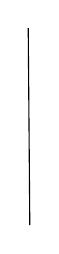
\begin{tikzpicture}[x=1cm,y=1cm]\draw (0,0)--(-0.02,2.5);\end{tikzpicture}}

Soit $\overline F$ l'ens de ces $A$. On a $F\subset\overline F$, $\overline{\overline F}=\overline F$. On voit que $\overline F$ satisfait a) b) c) d). \deleted{(satisfait-il e)?} Il n'est pas clair qu'il satisfait e), \deleted{\unsure{ainsi}} ni que $\overline F$ est engendré par les fermés qu'il contient.

Mais si $X$ est quasi-compact, on a $F=\overline F$ (car on peut prendre les $U_i$ en nb fini)

Si on ne suppose plus que la top. de $X$ soit engendrée par les ouverts $\in F$, on
\mspage{21}

\scanpage{21}
peut néanmoins définir $\Phi_F$, ses sections sur l'ouvert $U\subset X$ sont les $A\subset U$ tels que $\forall x\in U$, $\exists$ voisinage (ouvert \unsure{si on veut}) $V_x$ \inserted{et $B_x\in F$} tels que $A\cap V_x=B_x\cap V_x$. Ici encore $\overline F=\Gamma(X,\Phi_F)$ \inserted{(plus généralement, $\Gamma(U,\Phi_F)=\overline F_U$ si $U$ ouvert de $X$)} satisfait a) b) c) d) (\unsure{peut-être|sans doute} pas e), ni $\overline F$ engendré par ses fermés\ldots), mais \unsure{$=$|même} si $X$ compact, on ne peut affirmer que \deleted{$\unsure{\Phi|F}$} $\overline F=F$. Par contre, si $F=\{\varnothing,X\}$, alors $\overline F$ est formé des parties à la fois ouvertes et fermées de $X$ (donc si $X$ est loc connexe, ce sont \unsure{les|des} réunions de comp. connexes).

\deleted{\unsure{plus général$^t$|plus généralement}}

Supposons p.ex. que $F=F_{\mathcal P}$, où $\mathcal P$ est décomposition cellulaire de $X$. Quand aura-t-on $\overline F=F$? Toute partie ouverte et fermée d'une cellule fermée est $\in\overline F$, il \uline{faut} donc que les cellules fermées soient connexes. Si on veut plus généralement que pour $\underline{\forall}$ ouvert $U\subset X$, $U\in F$, $\overline F_U=F_U$, on voit de \unsure{$=$|même} qu'il faut que $\underline{\forall}$ les cellules soient connexes (puisque elles sont fermées dans un ouvert $U\in F$). Cela est-il suffisant pour que $\overline F_U=F_U$ pour \unsure{tt} $U$ ouvert $\in F$?
\mspage{22}

\scanpage{22}
On est ramené au cas $U=X$, soit $A$ qui est loc. une réunion de feuilles, l'est-il globalement? Il suffit de prouver que pour tte feuille $X_i$, telle que $X_i\cap A\ne\varnothing$, on a $X_i\subset A$, ou encore que $X_i\cap A$ est une partie à la fois ouverte et fermée de $A$. C'est une condition locale sur $X$, or loc. sur $X$ $A$ est \unsure{comme|connue} une réunion de feuilles, OK!

Cet argument montre plus gén. que pour \uline{tout} ouvert $U\subset X$, si $A\in\overline F_U$, alors les $A\unsure{\cap|\equiv} X_i$ sont à la fois ouverts et fermés dans $X_i\cap U$, donc des réunions des comp. connexes de $X_i\cap U$. \inserted{Donc $A$ est réunion de comp. connexes d'ens. \deleted{\unsure{ouverts}} de la forme $X_i\cap U$.} Inversement, supposons que $A$ soit une telle réunion, cela implique-t-il que $A\in\overline F_U$? \deleted{Evidemment, \unsure{les composantes}}\inserted{En particulier, une comp.} connexe d'un $X_i\cap U$ est-il $\in\overline F_U$?

\uuline{Non}, exemple:
\[
\begin{aligned}
&X=U=\text{droite numérique }\mathbb R\\
&\deleted{\unsure{F}=\{\varnothing,\mathbb R,\{0\},\mathbb R^*\}}\\
&X_0=\{0\},\quad X_1=\mathbb R^*=\mathbb R-\{0\}
\end{aligned}
\]
\figure{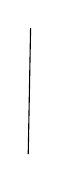
\begin{tikzpicture}[x=1cm,y=1cm]\draw (0,0)--(0.03,1.6);\end{tikzpicture}}
$\mathbb R^+$ n'est pas $\in\overline F=F_X$.

\figure{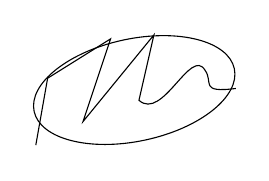
\begin{tikzpicture}[x=1cm,y=1cm]\draw[rotate=12] (0,0) ellipse (1.3 and .65);\draw (-1.25,-.7)--(-1.1,.15)--(-.3,.65)--(-.65,-.4)--(.25,.7)--(.06,-.13) .. controls (.36,-.4) and (.72,.56) .. (.9,.25) .. controls (1.01,.1) and (.82,-.04) .. (1.29,.02);\end{tikzpicture}}

Si on veut un exemple avec des $X_i$ connexes, $U\ne X$, on prend $X=\widehat{\mathbb R}=\unsure{\mathbb P^1_{\mathbb R}|\mathbb S^1}$; \deleted{$\unsure{U\in F}$} $X_0=\{0\}$, $X_1=X-\{0\}$, $U=\mathbb R$ ---
\mspage{23}

\scanpage{23}
Nous attachons maintenant notre attention à la condition f). \deleted{Il est clair}\inserted{On a vu} qu'elle \deleted{\unsure{est}} est stable par restriction à un ouvert $\in F$, mais il est assez clair qu'elle n'est pas stable par restriction à un ouvert quelconque. On a seulement, alors, que si $A\in\overline F_U$ est loc fermé dans $U$ (donc \unsure{l'est|fermé} dans un ouvert plus petit $V\subset U$), alors $A$ est loc. connexe, \deleted{et $\unsure{\overline F|F}$} donc ses comp. connexes sont ouvertes. Si $A$ est loc compact (p.ex. si $X$ l'est) alors ses comp. connexes \unsure{forment} donc une famille loc finie dans $A$ (donc dans $V$) \deleted{\unsure{mais est}} \uline{Elle} \inserted{\uline{est $=$}} \uline{\unsure{loc$^t$} finie dans} $U$?
\margin{Je suppose la top. de $X$ engendrée par les ouverts $\in F$}

\deleted{\unsure{Cela n'est que} au voisinage de tt pt de $U$, on a $A=\deleted{\unsure{Z\cap U}}$ avec $\deleted{\unsure{B}}Z\in F$ $Z$ loc. fermé,} car $\forall x\in U$, $\exists$ voisinage ouvert $V\in F_U$, tel que $A\cap V\in F$, et $A\cap V$ n'a qu'un nb fini de comp connexes.

\figure{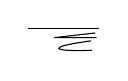
\begin{tikzpicture}[x=1cm,y=1cm]\draw (-.45,.12)--(.45,.12);\draw (.4,.06)--(-.12,0)--(.42,0);\draw (.35,-.04)..controls(-.25,-.12)and(-.15,-.18)..(.36,-.16);\end{tikzpicture}}

Soit $\underline F$ un sous-faisceau du faisceau $\underline{\mathcal P}_X$ des germes de parties de $X$. On suppose que $\underline F$ satisfait a) b) c) d), et \deleted{\unsure{que de plus une famille}} \inserted{e)} Soit $U$ un ouvert de $X$, et $X_1\supset X_2\supset\cdots\supset X_n\supset\cdots$ des fermés de $U$, $\in\Gamma(U,\underline F)$, tels que $X_{\unsure{n+2|n+1}}$ rare dans $X_n$. Alors la suite des $X_i$ est loc finie sur $U$, donc $\bigcap X_i=\varnothing$.
\mspage{24}

\scanpage{24}
(donc pour tt partie quasi-compacte $K$ de $U$, $\exists i=i(K)\in\mathbb N$ tel que $X_i\cap K=\varnothing$). Alors $F=\Gamma(X,\underline F)$ satisfait à a) b) c) d) \deleted{\unsure{e)}} et aussi à e) si $X$ quasi-compact. Plus \unsure{gén.}, si $A\in\unsure{F}$, alors $F_A$ \inserted{$=$ ens des parties de $A$ qui sont loc. \unsure{induites} par des sections de $\underline F$} satisfait à a) b) c) d) \deleted{\unsure{e)}} (il satisfait à e) si ???).

\unsure{Ici} il est plus commode de postuler l'axiome suivant plus fort que e)

$(e_n)$ $\exists$ un entier $n$ tel que si \inserted{$U,$} $X_0\supset X_1\supset\cdots\supset X_n\supset X_{n+1}$ est comme dans $\unsure{e)_{\underline F}|e)}$ ci-dessus, alors on a $X_{n+1}=\varnothing$. (On dit que $X$ est de $\underline F$-dim $\leq n$)
\figure{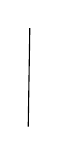
\begin{tikzpicture}\draw (0,0)--(.02,1.25);\end{tikzpicture}}
Alors tous les $F_A$ ($A$ \deleted{\unsure{loc$^t$}} fermé dans $X$) satisfont \deleted{\unsure{à}} $e_n)$, donc e).

\uline{NB} $\underline F$ est à priori $\supset$ le faisceau \uline{engendré} par $F=\Gamma(X,\underline F)$ et l'inclusion peut être stricte. \uline{Ex}: germes de parties analytiques d'un tore analytique de dim 2 sans fonctions méromorphes non constantes ---

Nous \deleted{\unsure{supposons}} \inserted{envisageons} maintenant une condition

f)
\mspage{25}

\scanpage{26}
1. $X$ espace top.

$Y$ sous-espace ``non singulier'' i.e. variété

$X$ est dit ``\uline{équisingulier le long de} $Y$'' si $\forall y\in Y$, \deleted{\unsure{alors}} $\exists$ espace pointé $(N,a)$, \deleted{et} un voisinage ouvert $U$ de $y$ dans $X$, et un homéom
\diagram{\begin{tikzcd}[column sep=1.4em]
{} & U \arrow[r,phantom,"\simeq"] & N\times\unsure{Y|V}_U & (Y_U=Y\cap U) \\
\text{avec commutativité:} & Y_U \arrow[u,hook] \arrow[r,"\simeq","\mathrm{can}"'] & a\times Y_U \arrow[u,hook] & {}
\end{tikzcd}}

On dit que $x\in X$ est une \uline{singularité élémentaire} \inserted{(ou \deleted{\unsure{spéciale}} \inserted{immobile})} de $X$ si $\forall Y\subset X$, $Y$ sous-espace \deleted{\unsure{de $X$}} non-singulier de $X$, $Y\ni x$, $X$ équisingulier \deleted{\unsure{sur $Y$}} le long de $\unsure{Y}$, on a $\dim_xY=0$.

On dit que $x\in X$ est une \uline{singularité} \uline{$\nu$-mobil\unsure{e}\deleted{\unsure{ité}}} \deleted{\unsure{élémentaire}}, si $\exists Y\subset X$ sous-espace, $Y$ non sing., $Y\ni x$, $X$ \inserted{équi}singulier le long de $Y$, $\dim_xY\geq\nu$.

(N.B. on peut alors choisir $Y$ avec $\dim Y=\nu$).

\deleted{Ainsi, les singularités \unsure{élémentaires}}

On dit que $x$ a un \uline{ordre de mobilité} $\nu$ si $x$ est $\nu$-mobile mais non $(\nu+1)$-mobile. (Ainsi les singularités élémentaires \inserted{ou ``immobiles''} sont celles qui sont d'ordre de mobilité 0). \deleted{Donc les points} \deleted{\unsure{L'ens des points qui ont un ordre de} $\nu$-mobiles,} \inserted{Les points qui ont un ordre de mobilité} $\nu\geq\nu_0$ ($\nu_0$ donné) sont les p\textsuperscript{ts} $\nu_0$-mobiles qui ont un ordre de mobilité. (Mais si $X$ \deleted{\unsure{a}} est loc de dim finie, tt p\textsuperscript{t} \inserted{$x$} de $X$ a nécessairement un ordre de mobilité \inserted{$\nu(x)$}, qui est le sup des dim en $x$ des ss-espaces de $X$ \deleted{\unsure{singuliers}} non singuliers \deleted{qui sont} le long desquels $X$ est équisingulier)
\mspage{27}

\scanpage{27}
\deleted{Supposons que $\nu(x)$ existe pour tt $x\in X$ (p.ex. $X$ loc. de dim finie)}
L'ens des p\textsuperscript{ts} $x\in X$ tels que \deleted{$\nu(x)\geq i$, est un} \inserted{$x$ soit $i$-mobile dans $X$} \inserted{est un} \uline{ouvert} \deleted{$\unsure{F|M}$} $\operatorname{Mob}^i(X)$ --- \unsure{on obtient un sys} décroissant
\[
\operatorname{Mob}^0(X)=X\supset\operatorname{Mob}^1(X)\supset\operatorname{Mob}^2(X)\supset\cdots
\]
\inserted{dont l'intersection est vide ssi $\forall x\in X$, $\nu(x)$ défini (p.ex. $X$ loc. de dim finie)}
Les complémentaires forment des \deleted{\unsure{pts}} ensembles
\[
F_0(X)\subset F_1(X)\subset F_{\unsure{3|2}}(X)\subset\cdots
\]
\[
(F_i(X)=X-\operatorname{Mob}^{i+1}(X))
\]
\margin{réunion des $F_i(X)$ est $X$ ssi $\forall x\in X$, $\nu(x)$ défini (p.ex. $X$ loc. de dim finie)}

Pour tout $X$ fixé, on se pose la question \deleted{suivante:} de la validité des propositions ``suivantes'' (où $F_{-1}(X)=\varnothing$)

\uline{Prop A} $\forall i\geq0$, $\deleted{\unsure{Y_i(X)|F_i(X)}}\inserted{Y_i=}F_i(X)-F_{i-1}(X)=\nu_{\unsure{X|\xi}}^{-1}(\{i\})$ (ens des p\textsuperscript{ts} d'ordre de mobilité $i$) est un sous espace non singulier purement de dimension $i$, et $X$ est équisingulier le long de $Y_i$.
\margin{Appelons espaces ``\unsure{dévissables}'' les espaces loc de dim finie pour lesquels \unsure{prop A soit|prop A est} vraie.}
\figure{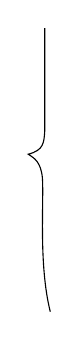
\begin{tikzpicture}\draw (.2,0)..controls(.05,.6)and(.12,1.4)..(.1,1.7)..controls(.08,1.9)and(0,1.95)..(-.08,2)..controls(.12,2.05)and(.12,2.15)..(.13,2.3)--(.13,3.6);\end{tikzpicture}}

\uline{Prop B} Localement au voisinage de chaque pt de $Y_i$, on a $(X,Y_i)\simeq Y_i\times(N_{\unsure{i|\xi}},a)$, où $\unsure{a|N}$ est un espace topologique dont $a$ est une singularité \uline{immobile}. [Le type d'homéomorphie locale de $(N,a)$ ne dépend que de la composante connexe du point envisagé de $Y_i$]
\margin{Vrai $\forall X$ \unsure{dévissable}, et alors \deleted{\unsure{alors}} $N$ est \unsure{dévissable}?}
\figure{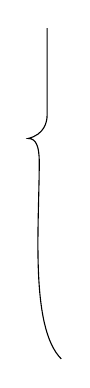
\begin{tikzpicture}\draw (.3,0)..controls(-.1,.4)and(.02,1.7)..(.02,2.5)..controls(.02,2.7)and(-.02,2.8)..(-.12,2.8)..controls(.08,2.85)and(.12,3)..(.12,3.1)--(.12,4.2);\end{tikzpicture}}

\uline{Prop C} Pour tt $x\in Y_i$, $(Y_i,\unsure{y|x})$ est le \deleted{\unsure{p}} plus gros germe de sous-variété \inserted{$Y$} de $X$ en $x$ le long de laquelle $X$ soit équisingulier. Tous les ``autres'' $Y$ correspondent \inserted{$\overset{1-1}{\longleftrightarrow}$} aux germes \inserted{en $x$ de} sous-variétés régulièrement immergées de $Y_i$. \deleted{\illegible{1}}
\mspage{28}

\scanpage{28}
\uline{Prop D} Soit $Y$ \deleted{\unsure{a}} une variété topologique purement de dim $i$, $N$ un espace topologique. Alors \deleted{\unsure{fixé|si}}, $\forall(y,n)\in Y\times N$, \deleted{\unsure{tt|et} $\nu(y,n)$ est \unsure{défini}} \deleted{$(y,n)$ est $\nu$-mobile ssi} Si $\nu\geq i$, $(y,n)$ \inserted{$\in Y\times N$} est $\nu$-mobile ssi $n\in N$ est $(\nu-i)$-mobile. Donc
\[
Y_{\nu}(Y\times N)=Y\times Y_{\nu-i}(N).
\]
\margin{\diagram{\begin{tikzcd}[row sep=1em]
N\text{ dévissable} \arrow[d,Leftrightarrow] & {} \\
Y\times N\text{ dévissable}\quad(Y\neq\varnothing) & {} \arrow[dl,Rightarrow] \\
\text{\uline{Prop B}} & {}\\
\text{(\unsure{sous|sans} réserve de Prop A)}
\end{tikzcd}}}
\figure{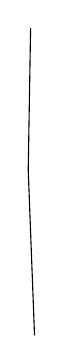
\begin{tikzpicture}\draw (0,0)--(-.08,2.1)--(-.05,3.9);\end{tikzpicture}}
\mspage{29}

\scanpage{30}
\uline{Équisingularité}

\deleted{\unsure{On}} Le contexte des ``espaces'' est celui des espaces topologiques, ou des espaces linéaires \inserted{(ou algébriques, ou \unsure{analytiques})} par morceaux. \deleted{ou des espaces algébriques \unsure{par|p.ex.}} \unsure{Les mots|Le mot} ``espace'' et ``flèche'' désignent des \deleted{\unsure{tels}} objets et morphismes du contexte choisi

Soient $X$ un espace, $Y$ un sous-espace loc. fermé. $X$ est dit \uline{équisingulier le long de $Y$} si $\forall y\in Y$, $\exists$ ouvert $X'$ de $X$, et espace pointé $(Z,a)$, tels que l'on ait un diagramme commutatif
\diagram{\begin{tikzcd}
X'\cap Y=Y'_{\unsure{a|u}} \arrow[r,hook] \arrow[d,"\unsure{\wr|2}"] & X' \arrow[d,"\unsure{\wr|2}"] \\
Y'\times\{a\} \arrow[r,hook] & Y'\times Z
\end{tikzcd}}

Plus généralement, soit $\mathcal X=(X_i)_{i\in I}$, un diagramme d'espaces ($I$ étant un type de diagramme, p.ex. défini par un ens. ordonné --- c'est le seul cas que nous aurons à envisager), soit $i_0\in I$ et $Y$ un sous-espace loc. fermé de $X_{i_0}$. On dit que $\mathcal X$ est \uline{équisingulier le long de $Y$} si, désignant par $J$ le sous-diagramme de $I$ formé de tous les $j\in I$ pour lesquels \inserted{ou bien $j=i_0$ ou bien} $\exists$ flèche $j\longrightarrow i_0$, $\forall y\in Y$ \unsure{peut|pourra} trouver un voisinage ouvert $X'_{i_0}$ de $y$ dans $X_{i_0}$, un diagramme \inserted{d'espaces} $(Z_j)_{j\in J}$, avec $Z_{i_0}$ muni d'un point $a\in Z_{i_0}$, et un \unsure{homomorphisme|homéomorphisme} des diagrammes (où $Y'=Y\cap X'_{i_0}$)
\diagram{\begin{tikzcd}
(Z_j\times Y')_{j\in J} \arrow[r] & (X_j)_{j\in J}
\end{tikzcd}}
tel que pour tout $j\in J$, $Z'_j\times Y' - X_j$ soit un plongement ouvert, et que $\exists$ diagramme comm.
\diagram{\begin{tikzcd}
Y' \arrow[r,hook] \arrow[d,no head,"\unsure{\wr|2}"] & X'_{i_0} \arrow[d,no head,"\unsure{\wr|2}"] \\
\{a\}\times Y' \arrow[r,hook] & Z_{i_0}\times Y'
\end{tikzcd}}
\mspage{31}

\scanpage{31}
Soit $X$ un espace, $(X_i)_{i\geq0}$ une filtration croissante (pour fixer les idées) de $X$ par des sous-espaces fermés. On dit que la \uline{filtration est équisingulière} si $\forall i\geq0$, le diagramme formé de
\diagram{\begin{tikzcd}
(\,X_0 \arrow[r] & X_1 \arrow[r] & \cdots \arrow[r] & X\,)
\end{tikzcd}}
est équisingulier le long de $X_i-X_{i-1}=V_i$.

(NB on pose $X_{-1}=\varnothing$).

Appelons ``feuille (\unsure{entrante})'' de la filtration toute composante connexe d'un $V_i=X_i-X_{i-1}$.
\margin{\unsure{1|?}}
Les feuilles \unsure{entrantes} forment donc une \uline{partition} de $X$ si $X$ est réunion des $X_i$, ce qu'on suppose désormais.

\uline{Proposition} Si la \deleted{\unsure{condition}} filtration est équisingulière, alors l'adhérence de toute feuille est une réunion de feuilles.

(Si $X$ est compact, et les $X_i$ loc. connexes --- ce qui est vrai dans le contexte lin. \unsure{ou} alg. ou an. ``par morceaux'' --- alors il s'agit bien sûr d'une réunion \uline{finie} de feuilles $\ldots$)

Les adhérences des feuilles sont appelées \uline{feuilles fermées}. Il y a corr. biunivoque par $F\longmapsto\overline F$ entre feuilles (\unsure{entrantes} --- on \unsure{ose} les appeler ``ouvertes'') et feuilles fermées. Les parties \uline{fermées} de $X$ qui sont réunions de feuilles sont aussi celles qui sont réunions de feuilles fermées; Toute intersection et toute réunion finie de telles parties est une
\mspage{32}

\scanpage{32}
partie du même type. Par exemple toute intersection de feuilles fermées est une réunion de feuilles fermées.

La relation d'inclusion entre feuilles fermées induit une relation d'ordre sur l'ens des feuilles, appelée ``relation d'incidence''. La réunion des feuilles incidentes à une feuille donnée $F$ et distinctes d'elle n'est autre que $\overline F-F$; on l'appelle le \uline{bord} de la feuille $F$; c'est \unsure{bien|donc} une partie fermée, réunion de feuilles fermées.

\uline{Proposition} Pour que la filtration donnée de $X$ soit équisingulière, il f. et s. qu'elle satisfasse les 2 conditions:

a) $\forall$ feuille $F$, $\overline F$ est une réunion de feuilles

b) Le diagramme formé de $X$ et de toutes les feuilles fermées (avec les applications d'inclusion) est \deleted{\unsure{constant près de|constant par le}} \inserted{équisingulier} le long de chaque feuille.

On dit qu'une partition $(F_i)_{i\in I}$ \deleted{de $X$} \inserted{d'un} espace $X$ \inserted{en ``feuilles'' $F_i$} est \deleted{\unsure{équi}} une \uline{partition équisingulière} si 1°) chaque $F_i$ est la différence de deux sous-espaces fermés (i.e. $\overline{F_i}$ et $\overline{F_i}-F_i=bF_i$ sont des sous-espaces fermés) 2°) Chaque $\overline{F_i}$ est une réunion de feuilles et 3°) le diagramme formé par \inserted{$X$,} les $\overline{F_i}$ et leurs inclusions est équisingulier le long de chaque feuille.
\margin{Si 1° et 2° sont satisfaites on dira que la partition est cellulaire}
\figure{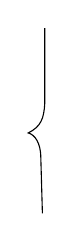
\begin{tikzpicture}\draw (0,0)--(-.02,.7)..controls(-.02,.9)and(-.1,1)..(-.18,1.02)..controls(-.02,1.1)and(.02,1.2)..(.03,1.4)--(.03,2.35);\end{tikzpicture}}
\mspage{33}

\scanpage{33}
\uline{NB} Deux filtrations \deleted{différentes}\inserted{équisingulières} de $X$ peuvent très bien définir des \deleted{filtrations} partitions identiques de $X$ en feuilles. C'est la partition en feuilles qui est le plus important, non la filtration.

P.ex. dans le contexte ``par morceaux'', où on dispose donc d'une notion de ``dimension'' et de ``codimension'', il y a au moins 4 façons canoniques, \deleted{\unsure{deux à deux}}\inserted{distinctes} ``en général'', pour décrire une partition équisingulière donnée à l'aide de filtrations : 1°) $X_i =$ réunion des feuilles de dimension $\leq i$, 2°) $X_0 =$ réunion des feuilles minimales $\ldots$ $X_i =$ réunion des feuilles minimales parmi celles qui sont $\notin X_{i-1}$, 3° et 4° définitions ``duales'' de 1° et 2°, donnant des filtrations \uline{décroissantes}.

Pour la suite, on préférera utiliser le langage des espaces à partitions équisingulières, plutôt que des espaces filtrés équisinguliers.

\inserted{\uline{Prop.} Si la partition donnée de $X$ est équisingulière, \unsure{de $=$} pour ttes les parties loc. fermées de $X$ qui sont réunions de feuilles, \deleted{\unsure{la partition}}\inserted{\unsure{induite}}\deleted{\unsure{est}} équisingulière.}

Soit $(X_i)_{i\in I}$ un diagramme d'espaces, et supposons que tout $X_i$ est muni d'une partition \deleted{admissible}. On \deleted{\unsure{en définit le}}\inserted{\unsure{dit qu'un|dit que ce}} système \deleted{\unsure{est dit}} de partitions est \uline{admissible} si

a) $\forall i\in I$, la partition donnée de $X_i$ est admissible

b) $\forall$ flèche $i\to j$, l'application $X_i\unsure{-|\to}X_j$ applique une feuille de $X_i$ dans une feuille (évidemment uniquement déterminée) de $X_j$.
\mspage{34}

\scanpage{34}
Lorsque cette condition est satisfaite, on définit un nouveau diagramme (dont le type se déduit de façon évidente du type de diagrammes $I$, des ensembles ordonnés par incidence \deleted{des} $\Phi_i$ des feuilles des espaces $X_i$, et des morphismes d'ensembles ordonnés \deleted{$\unsure{\Phi|\mathcal X}$} $\Phi_i\unsure{-|\to}\Phi_j$ définis par les \deleted{flèches} applications $X_i\to X_j$ définies par les flèches du diagramme $I$ -- d'où un diagramme \inserted{$(\Phi_i)_{i\in I}$} de type $I$ d'ensembles ordonnés $\ldots$), par les applications $\overline F_{i,\alpha}\unsure{-|\to}\overline F_{j,\beta}$ entre feuilles \uline{fermées} induites par les $X_i\unsure{-|\to}X_j$.

Ceci dit, le \deleted{système \unsure{diagramme}}\inserted{système} des partitions des $X_i$ est dit \uline{équisingulier} (relativement au diagramme donné $\mathcal X=(X_i)_{i\in I}$) si \inserted{\unsure{(il est admissible, et si)}} le diagramme \deleted{des}\inserted{précédent} \deleted{$\unsure{F}$} applications entre feuilles fermées est équisingulier le long de toute feuille (\unsure{entrante}) de tout $X_i$.

\margin{Un système de partitions est dit ``privilégié'' s'il est équisingulier et si de plus toutes les feuilles de tous les $X_i$ sont des \uline{variétés} (sans bord).}
\figure{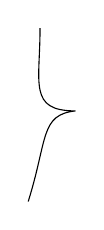
\begin{tikzpicture}[x=1cm,y=1cm]\draw (0,2.2) .. controls (0,1.5) and (-.15,1.15) .. (.45,1.15) .. controls (0,1.1) and (.1,.8) .. (-.15,0);\end{tikzpicture}}
\figure{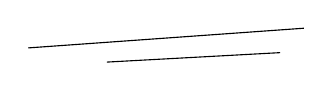
\begin{tikzpicture}[x=1cm,y=1cm]\draw (0,.18)--(3.5,.43);\draw (1,.0)--(3.2,.12);\end{tikzpicture}}

On suppose maintenant que le contexte soit linéaire (ou algébrique, ou analytique) par \uline{morceaux}.

\uline{Conjecture 1} Tout espace $X$ admet une partition \deleted{équisingulière}\inserted{privilégiée}. Parmi toutes les partitions \deleted{équisingulières}\inserted{privilégiées} de $X$, il en est une plus grossière que toutes les autres (appelée ``canonique'').
\mspage{35}

\scanpage{35}
Cela ne suffit pas pour bien des questions : on aura besoin de partitions privilégiées qui \deleted{\unsure{suff}} soient plus fines qu'une partition \inserted{admissible} donnée, \inserted{\deleted{\unsure{ou}}(\unsure{plus gross.})} ou telles que \deleted{\unsure{donnés}} pour des sous-espaces fermés \uline{donnés} \inserted{$X_i$} de $X$ en nb fini, chacun soit réunion de feuilles et que la filtration induite soit \deleted{équisingulière}\inserted{privilégiée}. Ou pour une application donnée $X\to Y$, on voudrait trouver simultanément des partitions privilégiées compatibles avec cette application. Tous ces cas \unsure{sembleraient|semblent avoir} couverts par l'énoncé conjectural suivant :

\uline{Conjecture 2} Soient $I$ un ens. ordonné \uuline{fini}, $(X_i)_{i\in I}$ un diagramme de type $I$ d'espaces, avec les applications $X_i\to X_j$ \uline{propres}. Alors il existe des partitions privilégiées de ce diagramme, et il y a parmi elles une moins fine (appelée comme de juste ``canonique'').

\uline{Remarque} Soit une \deleted{\unsure{filtr}} partition admissible pour un diagramme $(X_i)_{i\in I}$. Si $X_i\overset{f}{\unsure{-|\to}}X_j$ dans ce diagramme est \uline{propre}, on voit aussitôt que pour tte feuille $F_{\deleted{\unsure{\alpha}}}$ de $X_i$, s'appliquant \inserted{donc} dans une feuille $\Phi$ de $X_j$, l'image est $\Phi$ tout entier (et non seulement un ouvert de $\Phi$) \deleted{\unsure{car l'image}}\inserted{car l'image de} \deleted{\illegible{3}} $\overline F\cap f^{-1}(\Phi)$ est à la fois ouvert \inserted{dans $\Phi$}\deleted{\unsure{plus}}
\mspage{36}

\scanpage{36}
équisingularité) et fermé (par propreté) donc \uline{égal} à $\Phi$ qui est connexe; \deleted{et d'autre part} donc $\Phi-f(F)$ est une réunion d'images de feuilles \inserted{$(\subset\overline F\cap f^{-1}(\Phi))$} de $X_i$, donc ouvert dans $\Phi$, donc $f(F)$ est à la fois ouvert et fermé dans $\Phi$, donc $=\Phi$ ] De plus, \deleted{bien entendu} comme $F$ est fibré loc. trivial sur l'ouvert $f(F)$ de $\Phi$, \deleted{\unsure{et que}} (équisingularité) il est en fait fibré loc. trivial sur $\Phi$ tt entier. Mieux, $f^{-1}(\Phi)$ \deleted{est fibré} \uline{avec} \deleted{la}\inserted{sa} \uline{partition induite} est un fibré loc. trivial sur $\Phi$. Comme $F$ \deleted{et} et $\Phi$ sont des variétés, il s'ensuit que les fibres de $F$ sur $\Phi$ doivent aussi être des variétés ---

Dans la première lettre à A-Campo, j'ai donné une description conjecturale de la ``partition privilégiée canonique'' d'un espace $X$, en termes de points ``immobiles''. Voici une description conjecturale de la ``partition privilégiée'' d'une application \uline{propre} \deleted{$f$}
\[
f:X\to Y
\]
Pour simplifier, on suppose $Y$ compact, donc $X$ compact. On \deleted{\unsure{détermine par récurrence une}}\inserted{procède par récurrence sur $\dim Y$ pour} \deleted{filtration décroissante de} la construction. Considérons le plus grand ouvert $U$ de $Y$ tel que 1°) $U$ est non singulier, 2°) $X|U\unsure{-|\to}U$ est un fibré loc. trivial. \unsure{Il faut} prouver que $Y-U=Y'$ est un sous-espace (de la catégorie ``par morceaux'' envisagée) \uline{rare} (donc $\dim Y'<\dim Y$). Les composantes connexes de $Y-Y'$ seront les feuilles
\mspage{37}

\scanpage{37}
ouvertes de la partition \unsure{donnée|cherchée} de $Y$. Les feuilles de $X$ au dessus de celles-ci sont simplement les feuilles de la partition \inserted{privilégiée} canonique (intrinsèque) de $V=X|U$ (loc. sur $U$, c'est le produit de $U$ avec une feuille canonique d'une fibre). Si $\overline F_i$ sont ces feuilles, il faudra bien sûr que les $\Phi'_i=\overline F_i-V\cap\overline F_i=\overline F_i|Y'$ soient des réunions de feuilles de $X$.
\figure{\begin{tikzpicture}[x=1cm,y=1cm]\draw (.1,.65)--(0,.1) .. controls (-.1,-.08) and (.18,-.05) .. (.1,.1) -- (0,.16);\end{tikzpicture}}
\margin{\figure{\begin{tikzpicture}[x=1cm,y=1cm]\draw (.1,.65)--(0,.1) .. controls (-.1,-.08) and (.18,-.05) .. (.1,.1) -- (0,.16);\end{tikzpicture}} Il faut donc prouver que les $\overline F_i$ (donc les $\overline F'_i$) sont encore des ``espaces'' de notre Catégorie.}
Mais si $X'=X|Y'=X-V$ on est ramené à trouver la \deleted{\unsure{décomposition}}\inserted{partition canonique} pour $X'\unsure{-|\to}Y'$, mais $X'$ étant muni de plus des sous-espaces $\Phi'_i$ et de leurs intersections finies, tant qu'à faire. On gagne par hyp. de récurrence, à cela près qu'il aurait fallu partir non avec $X\unsure{-|\to}Y$, mais avec en plus une famille finie de sous-espaces fermés donnés de $X$. Pour paraphraser dans ce cas plus général la construction précédente, il faut simplement (remplaçant $X$ par $V$) pour un espace $X$ muni d'une famille \inserted{finie} de sous-espaces fermés, définir la \deleted{\unsure{sa}} partition privilégiée canonique (i.e. la plus grossière) pour ce système. \unsure{Or} la construction est probablement à faire en paraphrasant celle proposée dans la \inserted{$1^{\mathrm{re}}$} lettre à A Campo.
\mspage{38}

\scanpage{39}
\diagram{\begin{tikzcd}[column sep=large]
(\overset{\mathcal F}{Y} & \unsure{Z|I}\arrow[l,"p"']\arrow[r,hook,"{\substack{i\\\bullet}}"] & \overset{\mathcal G}{X})=\mathcal X
\end{tikzcd}}
\diagram{\begin{tikzcd}
p^*(\mathcal F)\arrow[r,"\alpha"]&i^*(\mathcal G)
\end{tikzcd}}
\[(\mathcal F,\mathcal G,\alpha)\]

\diagram{\begin{tikzcd}[column sep=small,row sep=small]
& Z\arrow[dl,"p"',""{name=pleg,near start}]\arrow[dr,hook,"i",""{name=ileg,near start}] &&\\
Y\arrow[dr,hook,"i'"'] &&X\arrow[dl,"p"'] & X-Z\arrow[l,hook,"\deleted{\unsure{j}}"']\arrow[dll,bend left=15,"q"]\\
&\mathcal X&&
\arrow[from=pleg,to=ileg,dashed,bend right=25]
\end{tikzcd}}

\[\deleted{\unsure{p_*(i^*\mathcal G)|p_*(\mathcal F)}}-\]
\[
i'_*(\mathcal F)=(\mathcal F,0,0)
\]
\[
i'^*(\deleted{\unsure{\{|\mathcal G}}\mathcal F,\mathcal G\deleted{\unsure{\}}},\alpha)=\mathcal F
\]
\[
p'_*(\mathcal G)=(p_*i^*\mathcal G,\mathcal G,\operatorname{can}:p^*p_*(i^{\unsure{*|!}}\mathcal G)\unsure{-|\to}i^{\unsure{*|!}}(\mathcal G))
\]
\[p'^*(\mathcal F,\mathcal G,\alpha)=\mathcal G\]
\[q_!(\mathcal G)=(\unsure{\Phi|0},\mathcal G,0)\]
\[q^!(\mathcal G)=\]

\[X_{I,J}=X_I-X_J\]
\[
\Sigma\supset\underbrace{I\supset J}_{\substack{\text{\unsure{J un certain}}\\\text{\unsure{pa.|nb.} d'él. max. de }I}}
\]

\diagram{\begin{tikzcd}
\partial X_\alpha\arrow[r,"\unsure{p_\alpha|P_\alpha}"]\arrow[d,"i_\alpha"]&\deleted{\unsure{X_\alpha,X_\beta}}\\
X_{\unsure{\alpha|0\alpha}}&
\end{tikzcd}}

\diagram{\begin{tikzcd}
X_{I,J}\arrow[r,"\alpha_{I,J/I',J'}"]&X_{I',J'}
\end{tikzcd}}
\[
\left\{\begin{array}{l}
\alpha_*,\alpha^*,\alpha_!,\alpha^!\\
K^\bullet_{X,\Lambda}\quad\text{complexe dualisant}
\end{array}\right.
\]
\figure{\begin{tikzpicture}[x=1cm,y=1cm]\draw (.15,.3) .. controls (.12,.15) and (.08,.1) .. (0,0)--(.1,-.04);\end{tikzpicture}}
\mspage{40}

\scanpage{41}
Fujii Guruji \unsure{Nichidatsu|Nichidathu}

$I$ ens ordonné fini

$\forall i\in I\qquad V_i^\circ$ variété à bord [bord vide si $i$ minimal)

\[
\forall(i,j)\in I\times I,\quad j<i\qquad
\underset{\substack{\text{sous-}\\\text{variété à bord}}}{\partial_jV_i^\circ}\subset\partial V_i^\circ
\]
\diagram{\begin{tikzcd}
\partial_jV_i^\circ\arrow[r]&V_j^\circ
\end{tikzcd}}
\uline{fibration}

fibres des variétés à bord (variétés \inserted{sans bord} si $j$ prédécesseur de $i$)

\diagram{\begin{tikzcd}
\partial V_i^\circ=\displaystyle\bigcup_{\substack{j\in\Phi_i\\\text{ens des facettes de }i}}\underbracket{\partial_jV_i^\circ}\arrow[dr] &\\
&V_j^\circ
\end{tikzcd}}
\[
\partial(\partial_jV_i^\circ)=[(\partial_jV_i^\circ)|\partial V_j^\circ]\cup
\underbracket{\partial_{\unsure{i|\ell}/j}(\partial_jV_i^\circ)}_{\substack{\text{fibré des}\\\text{bords}}}
\]
\[
\partial(\partial_jV_i^\circ)=\bigcup_{k\in\Phi_j}\underbracket{(\partial_jV_i^\circ)|\partial_kV_j^\circ)}_{\text{fibré sur }V_k^\circ}
\cup\underbracket{\partial_{i/j}(\partial_jV_i^\circ)}_{\substack{\text{fibré sur}\\V_j^\circ}}
=\left(\bigcup_{k<j}\underbrace{(\partial_jV_i^\circ|\partial_kV_j^\circ)}_{\text{fibré sur }V_{\unsure{k|h}}^\circ}\right)
\cup\underbracket{\partial_{\unsure{0|i}/(j)}\partial V_i^\circ}_{\text{fibré sur }V_j^\circ}
\]
\figure{\begin{tikzpicture}[x=1cm,y=1cm]\node[draw,ellipse] at (0,0) {\unsure{bien|bon}};\node[anchor=west] at (.65,0) {vide si $j$ prédécesseur de $i$};\end{tikzpicture}}
\[
\partial(\partial_{j'}V_i^\circ)=\left(\bigcup_{k<j'}\partial_{j'}V_i^\circ|\partial_kV_{\unsure{j'|j}}^\circ\right)\cup
\underbracket{\partial_{i/j'}V_i^\circ}_{\substack{\text{vide si }j'\text{ préd.}\\\text{de }i}}
\]

\deleted{$\unsure{V_0|\partial_0}$}
\diagram{\begin{tikzcd}[column sep=large,row sep=small]
V_0^\circ&V_1^\circ&V_2^\circ\\
&\partial V_1^\circ\arrow[ul]&\partial V_2^\circ\arrow[d,equal]\\
&&\partial_1V_2^\circ\cup\partial_0V_2^\circ\arrow[uul,bend left=20]\arrow[uull,bend left=65]
\end{tikzcd}}
\[
\partial(\partial_0V_2^\circ)\simeq\partial(\partial_1V_2^\circ)=\partial_1V_2^\circ|\partial V_1^\circ
\]
\[
\partial_jV_i^\circ|\partial_kV_j^\circ=\partial_{j,\unsure{k|h}}V_i^\circ\qquad\text{fibré sur }V_{\unsure{h|k}}^\circ
\]
\figure{\begin{tikzpicture}[x=1cm,y=1cm]\draw[densely dashed] (0,.2)--(.65,.2);\draw[densely dashed] (.1,0)--(.8,0);\draw[densely dashed] (1.2,0)--(1.8,0);\draw (2.3,.02)--(2.4,-.02)--(2.5,0);\end{tikzpicture}}
\[
\partial_{j\unsure{>|,}h>\ell}=\partial_{j,h}V_i^\circ|\partial_\ell V_h^\circ\qquad\text{fibré sur }V_\ell^\circ
\]
\[
\partial_{j>h>\ell>m}V_i^\circ
\]

\diagram{\begin{tikzcd}[column sep=small,row sep=large]
\partial_2&\partial_{21}\arrow[l]\arrow[dr]&\partial_{20}\arrow[ll,bend right=50]\arrow[ll,bend left=20]\arrow[ddl,bend right=25]&\partial_{210}\arrow[l]\arrow[ll,bend right=50]\arrow[d,equal,"\text{bord commun}"]\\
\partial_1&\partial_{10}\arrow[l]\arrow[d,bend left=35]&\overset{\bullet\,\cdot}{\partial_{\deleted{\unsure{0}}\unsure{12|012}}}\arrow[ll,bend left=20]&\partial_{10}\arrow[l]\arrow[lll,bend left=40]\\
\partial_0&\deleted{\unsure{\partial}}\partial_0^\bullet\arrow[l]&&\text{bord commun}
\end{tikzcd}}

\figure{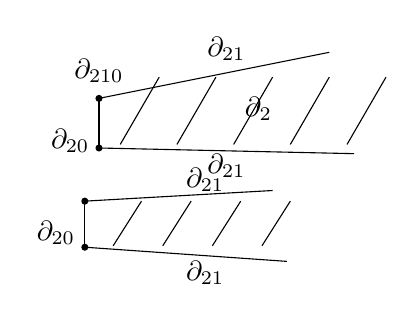
\begin{tikzpicture}[x=1cm,y=1cm,scale=.9]
\draw (0,2.8)--(3.25,3.45);\draw (0,2.1)--(3.6,2.02);\draw (0,2.8)--(0,2.1);
\foreach \x in {.3,1.1,1.9,2.7,3.5}{\draw (\x,2.15)--(\x+.55,3.1);}
\fill (0,2.8) circle(.05);\fill (0,2.1) circle(.05);
\node[above] at (0,2.88) {$\partial_{210}$};\node[left] at (0,2.2) {$\partial_{20}$};\node[above] at (1.8,3.2) {$\partial_{21}$};\node at (2.25,2.65) {$\partial_2$};\node[below] at (1.8,2.15) {$\partial_{21}$};
\draw (-.2,1.35)--(2.45,1.5);\draw (-.2,.7)--(2.65,.5);\draw (-.2,1.35)--(-.2,.7);
\foreach \x in {.2,.9,1.6,2.3}{\draw (\x,.72)--(\x+.4,1.35);}
\fill (-.2,1.35) circle(.05);\fill (-.2,.7) circle(.05);
\node[left] at (-.2,.9) {$\partial_{20}$};\node[above] at (1.5,1.35) {$\partial_{21}$};\node[below] at (1.5,.64) {$\partial_{21}$};
\end{tikzpicture}}

\figure{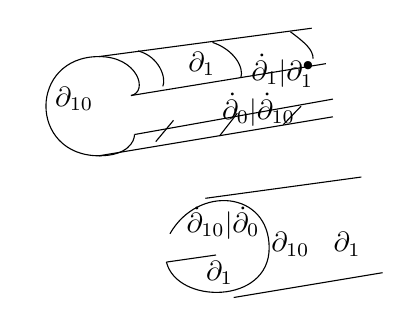
\begin{tikzpicture}[x=1cm,y=1cm,scale=.9]
\draw (0,2.4) .. controls (-1,2.4) and (-1,1) .. (0,1) .. controls (.4,1) and (.5,1.2) .. (.5,1.3);
\draw (0,2.4) .. controls (.55,2.4) and (.7,1.9) .. (.45,1.85);
\draw (0,2.4)--(3,2.8);\draw (.45,1.85)--(3.2,2.3);\draw (.5,1.3)--(3.3,1.8);\draw (0,1)--(3.3,1.55);
\draw (.55,2.48) .. controls (.85,2.4) and (.95,2.1) .. (.9,1.98);\draw (1.6,2.6) .. controls (1.9,2.5) and (2.05,2.25) .. (2,2.1);\draw (2.7,2.75) .. controls (2.9,2.6) and (3.02,2.5) .. (3.02,2.37);
\draw (.8,1.2)--(1.05,1.5);\draw (1.7,1.28)--(1.95,1.6);\draw (2.6,1.44)--(2.85,1.7);
\node at (-.35,1.8) {$\partial_{10}$};\node at (1.45,2.3) {$\partial_1$};\node at (2.6,2.2) {$\unsure{\dot\partial_1|\partial_1^\bullet}$};\node at (2.25,1.65) {$\unsure{\dot\partial_0|\dot\partial_{10}}$};
\draw (1,-.1) .. controls (1.4,.6) and (2.4,.5) .. (2.4,-.3) .. controls (2.4,-1.1) and (1.1,-1.1) .. (.95,-.5);
\draw (.95,-.5)--(1.65,-.4);\draw (1.5,.4)--(3.7,.7);\draw (1.9,-1)--(4,-.65);
\node at (1.75,.05) {$\unsure{\dot\partial_{10}|\dot\partial_0}$};\node at (1.7,-.65) {$\deleted{\unsure{\partial_1}}$};\node at (2.7,-.25) {$\partial_{10}$};\node at (3.5,-.25) {$\partial_1$};
\end{tikzpicture}}

\figure{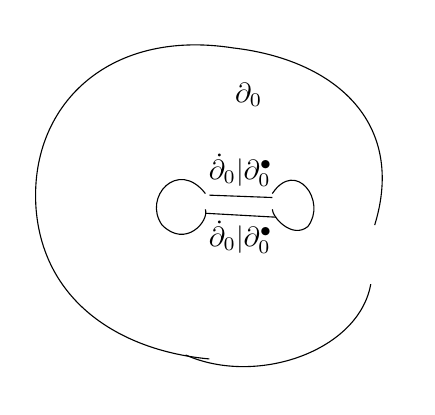
\begin{tikzpicture}[x=1cm,y=1cm]
\draw (3.8,2.1) .. controls (4.2,3.4) and (3.3,4.2) .. (2,4.35) .. controls (.4,4.6) and (-.6,3.6) .. (-.5,2.3) .. controls (-.4,1.1) and (.6,.5) .. (1.7,.4);
\draw (1.4,.45) .. controls (2.3,.05) and (3.6,.5) .. (3.75,1.35);
\draw (1.65,2.5) .. controls (1.3,2.95) and (.85,2.45) .. (1.1,2.1) .. controls (1.4,1.8) and (1.7,2.15) .. (1.65,2.3);
\draw (2.5,2.5) .. controls (2.8,2.95) and (3.2,2.4) .. (2.95,2.08) .. controls (2.75,1.92) and (2.5,2.2) .. (2.5,2.3);
\draw (1.7,2.48)--(2.5,2.45);\draw (1.65,2.25)--(2.55,2.2);
\node at (2.2,3.75) {$\partial_0$};\node at (2.1,2.8) {$\unsure{\dot\partial_0|\partial_0^\bullet}$};\node at (2.1,1.95) {$\unsure{\dot\partial_0|\partial_0^\bullet}$};
\end{tikzpicture}}

\figure{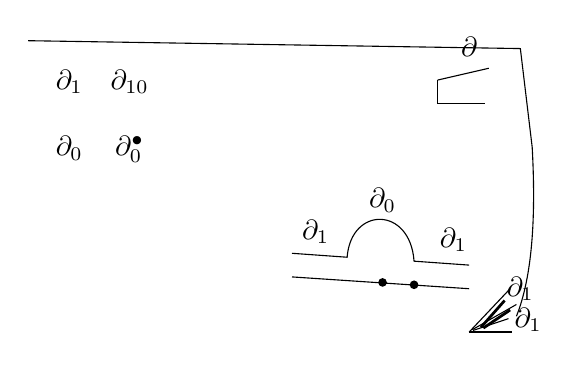
\begin{tikzpicture}[x=1cm,y=1cm]
\draw (0,3.8)--(6.25,3.7)--(6.4,2.45)..controls(6.45,1.55)and(6.4,.8)..(6.2,.3);
\node[anchor=north west] at (.05,3.6) {$\begin{array}{cc}\partial_1&\partial_{10}\\&\shortparallel\\\partial_0&\partial_0^\bullet\end{array}$};
\draw (5.2,3.3)--(5.85,3.45);\draw (5.2,3.3)--(5.2,3.0)--(5.8,3.0);\node[above] at (5.6,3.48) {$\partial$};
\draw (3.35,1.1)--(4.05,1.05)..controls(4.1,1.7)and(4.85,1.7)..(4.9,1.0)--(5.6,.95);\draw (3.35,.8)--(5.6,.65);
\fill (4.5,.73) circle(.055);\fill (4.9,.7) circle(.055);
\node[above] at (3.65,1.1) {$\partial_1$};\node[above] at (4.5,1.5) {$\partial_0$};\node[above] at (5.4,1) {$\partial_1$};
\draw (5.6,.1)--(6.15,.1);\draw (5.6,.1)--(6.12,.65);\draw (5.64,.13)--(6.2,.45);\draw (5.65,.12)--(6.1,.27);\draw[line width=1pt] (5.75,.16)--(6.05,.5);\draw[line width=1pt] (5.78,.15)--(6.12,.38);
\node at (6.25,.65) {$\partial_1$};\node at (6.35,.25) {$\deleted{\unsure{\partial_1}}$};
\end{tikzpicture}}
\mspage{42}

\scanpage{42}
\figure{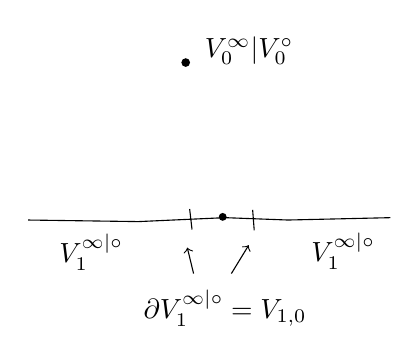
\begin{tikzpicture}[x=1cm,y=1cm]
\fill (0,2) circle(.055);\node[anchor=west] at (.12,2.15) {$\unsure{V_0^\infty|V_0^\circ}$};
\draw (-2,0)--(-.6,-.02)--(.5,.03)--(1.3,0)--(2.6,.03);
\draw (.05,.14)--(.08,-.12);\draw (.85,.13)--(.87,-.13);\fill (.47,.04) circle(.05);
\node[below] at (-1.2,-.05) {$V_1^{\unsure{\infty|\circ}}$};\node[below] at (2,-.04) {$V_1^{\unsure{\infty|\circ}}$};
\node at (.5,-1.12) {$\partial V_1^{\unsure{\infty|\circ}}=V_{1,0}$};
\draw[->] (.1,-.68)--(.02,-.35);\draw[->] (.58,-.68)--(.8,-.32);
\end{tikzpicture}}

\diagram{\begin{tikzcd}
\partial V_1=V_{10}\arrow[r]\arrow[d]&V_0\\
V_1&
\end{tikzcd}}

\figure{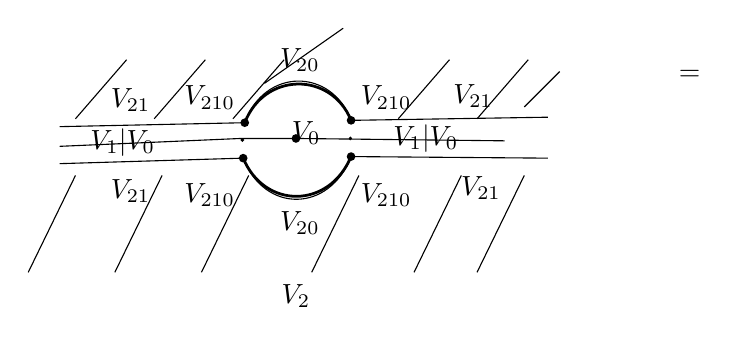
\begin{tikzpicture}[x=1cm,y=1cm]
\draw (-3,1.15)--(-.65,1.2).. controls(-.4,1.9)and(.45,1.9)..(.7,1.23)--(3.2,1.27);
\draw[line width=1pt] (-.65,1.2)..controls(-.4,1.85)and(.45,1.85)..(.7,1.23);
\draw (-3,.9)--(-.7,1.0)--(0,1.0)--(2.65,.97);
\draw (-3,.68)--(-.67,.75)..controls(-.4,.05)and(.42,.05)..(.7,.77)--(3.2,.75);
\draw[line width=1pt] (-.67,.75)..controls(-.4,.1)and(.42,.1)..(.7,.77);
\foreach \x in {-2.8,-1.8,-.8,1.3,2.3}{\draw (\x,1.25)--(\x+.65,2.0);}
\draw (-.4,1.7)--(.6,2.4);\draw (2.9,1.4)--(3.35,1.85);
\foreach \x in {-2.8,-1.7,-.6,.8,2.1,2.9}{\draw (\x,.53)--(\x-.6,-.7);}
\foreach \p in {(-.65,1.2),(.7,1.23),(-.67,.75),(.7,.77),(0,1.0)}{\fill \p circle(.055);}
\fill (-.68,.98) circle(.025);\fill (.69,1.0) circle(.025);
\node[above] at (-2.1,1.22) {$V_{21}$};\node[above left] at (-.65,1.25) {$V_{210}$};\node[above] at (.05,1.72) {$V_{20}$};\node[above right] at (.7,1.25) {$V_{210}$};\node[above] at (2.25,1.27) {$V_{21}$};
\node at (-2.2,.95) {$\unsure{V_1|V_0}$};\node at (.13,1.07) {$V_0$};\node at (1.65,1.0) {$\unsure{V_1|V_0}$};
\node[below] at (-2.1,.6) {$V_{21}$};\node[below left] at (-.65,.55) {$V_{210}$};\node[below] at (.05,.2) {$V_{20}$};\node[below right] at (.7,.55) {$V_{210}$};\node[below] at (2.35,.64) {$V_{21}$};\node at (0,-1) {$V_2$};\node at (5,1.8) {$\unsure{=}$};
\end{tikzpicture}}
\mspage{43}

\scanpage{43}
\diagram{\begin{tikzcd}[column sep=small,row sep=small]
F_0&F_1&\partial F_1=F_1|\partial\Phi_1&\\
|[draw,ellipse]|\Phi_0&|[draw,ellipse]|\Phi_1&\partial\Phi_1\arrow[l,"\unsure{i_1|\iota_1}"']\arrow[d,"\pi_1"{draw,ellipse}]&\\
&&\Phi_0&F_0\arrow[uul,bend right=35,"\unsure{\varphi|q}"']
\end{tikzcd}}

\diagram{\begin{tikzcd}[column sep=small,row sep=small]
F_2&\partial F_2=F_{\unsure{2|3}}|\partial\Phi_2&&\\
|[draw,ellipse]|\overset{\deleted{\unsure{\Phi}}}{\Phi_2}&\partial\Phi_2\arrow[l,"i_2"']&&\\
&|[draw,ellipse]|\partial_0\Phi_2\arrow[u,"\alpha_0"]&|[draw,ellipse]|\partial_1\Phi_2\arrow[ul,"\alpha_1"']&\\
&&|[draw,ellipse]|(\partial_1\Phi_2)_0\arrow[u,"\beta_0"]&|[draw,ellipse]|(\partial_1\Phi_2)_1\arrow[ul,"\unsure{\beta_1|\varphi_1}"']\\
&(\partial_0F_2)&\partial_1F_2&\\
&&(\partial_1F_2)_0&(\partial_1F_2)_1
\end{tikzcd}}
\figure{\begin{tikzpicture}[x=1cm,y=1cm]\draw (0,1.2)--(.8,1.15)..controls(2,1)and(1.5,.2)..(2.3,.1)--(2.8,0);\end{tikzpicture}}

\diagram{\begin{tikzcd}[column sep=small,row sep=large]
\partial_0\Phi_2\arrow[d,"{(\pi_2)_0}"'{draw,ellipse}]&(\partial_1\Phi_2)_0\arrow[dl,"{\substack{\deleted{\unsure{\pi_{2,0}}}\\(\pi_2)_{1,0}\\\deleted{\unsure{\pi}}}}"{draw,ellipse}]&(\partial_1\Phi_2)_1\arrow[d,"{\pi_{2,1,\unsure{2|1}}}"{draw,ellipse}]&\partial(\partial_1\Phi_2)_1\arrow[ll,bend right=35,"\pi'_1"']\arrow[d,"{\deleted{\unsure{\pi_{2,1,0}}}\ \partial\pi_{2,1,1}}"]\\
\Phi_0&&\Phi_1&\partial\Phi_1\arrow[lll,bend left=35,dash,"\unsure{\bar\pi_1|\pi_1}"']
\end{tikzcd}}
\figure{\begin{tikzpicture}\draw[line width=1pt] (0,0)--(.35,-.08);\draw[densely dashed](-.45,-.4)--(-.45,-.8);\end{tikzpicture}}

\diagram{\begin{tikzcd}[column sep=small,row sep=large]
\unsure{X_2|X_0}&&&&\\
X_1\arrow[u]&&&&\\
X_0=\boxed{\Phi_0}\arrow[u]&\boxed{\Phi_1}\arrow[ul]&\boxed{\Phi_2}\arrow[uull]&&\\
&\partial\Phi_1\arrow[u,"\square"{description}]\arrow[ul,"\circ"{description}]&\partial\Phi_2\arrow[u]\arrow[uull]&&\\
&&\boxed{(\partial_0\Phi_2)}\arrow[u]\arrow[uull,bend left=35,"\circ"{description}]&(\partial_1\Phi_2)\arrow[ul]&\\
&&&\boxed{(\partial_1\Phi_2)_0}\arrow[u]\arrow[uuulll,bend left=35,"\circ"{description}]\arrow[dl,equal]&\boxed{(\partial_1\Phi_2)_1}\arrow[ul]\arrow[uuulll,bend right=35,"\circ"{description}]\arrow[dr,equal]\\
&&\Psi_0&&\partial(\partial_1\Phi_2)_1\arrow[u,"\square"{description}]\arrow[ul,"\circ"{description}]&\Psi_1
\end{tikzcd}}

\diagram{\begin{tikzcd}[column sep=small,row sep=large]
\Phi_0&\Phi_1&\Phi_2&&\\
&\partial\Phi_1\arrow[u]\arrow[ul]&&&\\
&&\partial_0\Phi_2\arrow[uu]\arrow[uull,bend left=15]&(\partial_1\Phi_2)_0\arrow[uul]\arrow[uulll,bend left=40,dash]&(\partial_1\Phi_2)_1\arrow[uull]\arrow[uulll,bend right=50]\\
&&&&\partial(\partial_1\Phi_2)_1\arrow[u]\arrow[ul]\arrow[uulll,bend left=45]
\end{tikzcd}}

\diagram{\begin{tikzcd}[column sep=small,row sep=large]
\Phi_0\ \text{ens fini}&\Phi_1=\{&\Phi_1^\circ,\arrow[ll,bend left=25]\arrow[d]&\Phi_1^b\arrow[d]&\}\\
&&\begin{array}{l}\deleted{\unsure{groupe}\ \illegible{1}}\\\deleted{\unsure{holonomie}}\\\deleted{\unsure{des|les}\ \unsure{points|feuillets}}\\\deleted{\unsure{triviaux}\ \unsure{isolés}}\\\unsure{\mathbb Z/n\mathbb Z|\mathbb Z/2}\text{-torseur}\\\text{(}\unsure{\text{arêtes}|\text{orbites}}\ \unsure{\text{orientées}|\text{orientés}}\\\unsure{\text{reli-aires}}\text{)}\end{array}&\begin{array}{l}\deleted{\unsure{c}}\unsure{\text{gr-poïde}|\text{groupoïde}}\\\text{1-spécial}\\\deleted{\unsure{\text{connexe}}}\end{array}&\\
&&&\partial_0\Phi_2\subset\pi_0\mathcal F\arrow[uulll,bend left=55]&
\end{tikzcd}}

\diagram{\begin{tikzcd}[column sep=small,row sep=large]
\Phi_2=\{&\mathcal F\arrow[r,"i"{name=i}]\arrow[d]&\mathcal G\arrow[dr,bend right=20]&\}\ \deleted{\unsure{\mathcal G}}\\
&\begin{array}{l}\unsure{\text{gr-poïde}|\text{groupoïde}}\ \text{1-spécial}\\\deleted{\unsure{\text{connexe}}}\end{array}&&\begin{array}{l}\unsure{\text{gr-poïdes}|\text{groupoïdes}}\\\unsure{\text{2-espèces}|\text{2-spéciaux}}\end{array}\\
&&\begin{array}{l}\text{foncteurs}\\\text{admissibles}\end{array}\arrow[from=i,to=3-3,bend right=20]&
\end{tikzcd}}

\diagram{\begin{tikzcd}[column sep=small]
\Psi_0=\text{ens fini},&\Psi_1=\{\Psi_1^\circ,\Psi_1^b\}\arrow[l,bend left=25]
\end{tikzcd}}
\mspage{44}

\scanpage{44}
\diagram{\begin{array}{cccc}
&U&\subset V&\subset W\\
\deleted{\text{dim}}&&&\\
\text{dim:}&r&r+s&r+s+t
\end{array}}

$U$ \deleted{\unsure{est}} régulier

$V-U$ régulier

$W-V$ \deleted{\unsure{est}} régulier

$(V,W)$ \unsure{équisinguliers|équisingulier} le long de $\unsure{U}$

$W$ équisingulier le long de $V-U$

reconstruction

\deleted{$1^\circ$ \unsure{$U$} \unsure{espace}}

$1^\circ)$ $U$ espace régulier (dim $r$)

$2^\circ)$ $U'$ fibré sur $U$, fibres régulières (de dim $s-1$) donc $U'$ régulier

$3^\circ)$ $V^\circ$ variété à bord, de bord $U'$ (dim $r+s$)

$4^\circ)$ $V^{\circ\prime}$ fibré sur $V^\circ$, \deleted{des} fibres régulières (de dim $t-1$)

(sa dim est $r+s+t-1$), son bord est
\[
V^{\circ\prime}|\partial V^\circ=V^{\circ\prime}|U'
\]
(de dim $r+s+t-2$), fibré sur $U$: fibres régulières

$5^\circ)$ $U''$ autre fibré sur $U$ \inserted{(dim $r+s+t-1$)}, à fibres des \deleted{espaces réguliers} \inserted{variétés} à bord \inserted{(de dim $s+t-1$)} donc $\partial U''=$ fibré des bords (de dim $r+s+t-2$, fibres de dim $s+t-2$)

\margin{\diagram{\begin{tikzcd}[column sep=small,row sep=small]
&&V'=\partial W^\circ\unsure{\hookrightarrow|\subset} W^\circ\\
U''\arrow[dd]\arrow[urr,bend left=25]&\partial U''\arrow[l,hook]\arrow[d,equal]&\\
&\partial V^{\circ\prime}\arrow[r,hook]\arrow[d]&V^{\circ\prime}\arrow[uu,bend right=10]\arrow[d]\\
U&U'\arrow[l]\arrow[r,hook]\arrow[d,equal]&V^\circ\\
&\partial V^\circ&
\end{tikzcd}}
\figure{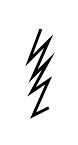
\begin{tikzpicture}[x=1cm,y=1cm]\draw[line width=1pt] (0,1.3)--(-.15,.9)--(.1,1.15)--(-.1,.7)--(.1,.9)--(-.12,.5)--(.1,.65)--(-.1,.2)--(.1,.3);\end{tikzpicture}}}

$6^\circ)$ Un isom. de $U$-fibrés en fibres régulières
\[
\partial U\unsure{=|\simeq}\partial V^{\prime\circ}
\]

On en conclut, par recollement, un \deleted{\unsure{variété sa}} espace régulier
\[
V'\deleted{\unsure{U}}=V^{\circ\prime}\amalg_{\partial V^{\circ\prime}=\partial U''}U''
\]

$7^\circ)$ \deleted{espace} \inserted{variété à bord} $W^\circ$, de bord $V'$

\figure{\begin{tikzpicture}[x=1cm,y=1cm]\draw (0,5.6)..controls(1.5,5.7)and(3,5.65)..(4.2,5.6)..controls(4.4,5.1)and(3.9,4.7)..(4.2,4.1)..controls(4.5,3.5)and(4.3,3.1)..(4.3,2.7)--(3.65,2.1)..controls(3.25,1.6)and(3.1,1)..(2.8,.8)..controls(1.4,.7)and(.3,.6)..(-.2,.4);\end{tikzpicture}}

On construit

\margin{\diagram{\begin{tikzcd}[column sep=small,row sep=small]
&&W^\circ\arrow[d,-{Hooks[harpoon]}]\\
&&V'=\partial W^\circ\\
\deleted{\unsure{U''}}\arrow[urr]&\deleted{\unsure{\partial U''}}\arrow[l,hook]&\\
U''\arrow[d]&\partial U''=\partial V^{\circ\prime}\arrow[l,hook]\arrow[r,hook]\arrow[d,"\text{cart}"']&V^{\circ\prime}\arrow[uu,hook]\arrow[d]\\
U&U'\arrow[l]\arrow[r,hook]\arrow[d,equal]&V^\circ\\
&(\partial V^\circ)&
\end{tikzcd}}}

$a)$ \deleted{\unsure{$U$}} $V=V^\circ\amalg_{U'}U$ et $U\hookrightarrow V$,
\diagram{\begin{tikzcd}[column sep=small,row sep=small]
&\unsure{V'|V''}\arrow[rrr]\arrow[d,equal]&&&V\arrow[d,equal]&\\
V^{\circ\prime}\arrow[rrr,bend right=40]&\amalg_{\partial}\arrow[rrr,bend right=55]&U''\arrow[rrr,bend right=35]&V^\circ&\amalg_{U'}&U
\end{tikzcd}}

\deleted{$b)\quad W=W^\circ\amalg$}

$b)$ $W=W^\circ\amalg_{V'}V$ et $V\longrightarrow W$
\mspage{45}

\scanpage{45}
\diagram{\begin{tikzcd}[column sep=small,row sep=large]
U_0\arrow[r,phantom,"\subset"]&U_1\arrow[r,phantom,"\subset"]\arrow[dl,-{Hooks[harpoon]}]&U_2\arrow[d,-{Hooks[harpoon]}]&&U_3\arrow[d,-{Hooks[harpoon]}]\\
U_1^\circ\ \unsure{\subset}\arrow[d,-{Hooks[harpoon]}]&&U_2^\circ\arrow[d,-{Hooks[harpoon]}]&&U_3^\circ\arrow[d,-{Hooks[harpoon]}]\\
\partial U_1^\circ=U'_0\arrow[uu,bend left=30]&&\partial U_2^\circ\arrow[dl,-{Hooks[harpoon]}]\arrow[dr,-{Hooks[harpoon]}]&&\partial U_3^\circ\arrow[d,-{Hooks[harpoon]}]\\
&U_1^{\circ\prime}\arrow[uul,bend right=20]\arrow[dr,-{Hooks[harpoon]}]&&U''_0\arrow[uuulll,bend right=45]\arrow[dl,-{Hooks[harpoon]}]&U_2^{\circ\prime}\arrow[uull,bend right=20]\arrow[d,-{Hooks[harpoon]}]\\
&&\partial U_1^{\circ\prime}=\partial U''\arrow[uull,bend left=25]&&\partial U_2^{\circ\prime}\arrow[uull,bend right=15]
\end{tikzcd}}

\diagram{\begin{tikzcd}[column sep=small,row sep=small]
&U_n\arrow[d]&&\\
&U_n^\circ\arrow[d,-{Hooks[harpoon]}]&&\\
&\partial U_n^\circ\arrow[dl,-{Hooks[harpoon]}]\arrow[d,-{Hooks[harpoon]}]\arrow[drr,bend left=15,-{Hooks[harpoon]}]&&\\
\partial_{n-1}U_n^\circ\arrow[d]&\partial_{n-2}U_n^\circ\arrow[d]&\cdots&\partial_0U_n^\circ\arrow[d,-{Hooks[harpoon]}]\\
U_{n-1}^\circ&U_{n-2}^\circ&&U_0^\circ=U_0
\end{tikzcd}}

\figure{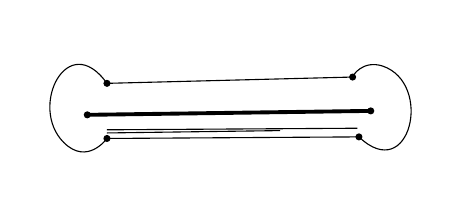
\begin{tikzpicture}[x=1cm,y=1cm]
\draw (0,.4)..controls(-.5,1.1)and(-1,.1)..(-.55,-.35)..controls(-.25,-.65)and(0,-.3)..(0,-.3)--(3.2,-.28)..controls(3.85,-.9)and(4.15,.4)..(3.5,.62)..controls(3.25,.7)and(3.12,.5)..(3.12,.48)--(0,.4);
\draw[line width=1.4pt] (-.25,0)--(3.35,.05);\draw (0,-.19)--(3.18,-.17);\draw (0,-.23)--(2.2,-.2);
\foreach \p in {(-.25,0),(0,.4),(0,-.3),(3.35,.05),(3.12,.48),(3.2,-.28)}{\fill \p circle(.045);}
\end{tikzpicture}}

\figure{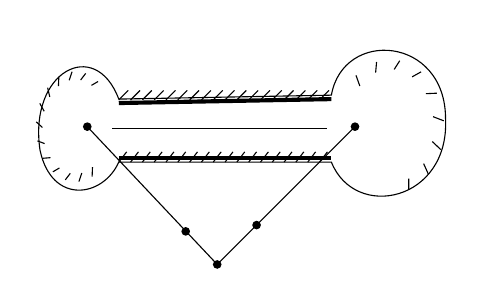
\begin{tikzpicture}[x=1cm,y=1cm]
\draw (0,.45)..controls(-.3,1.25)and(-1.15,.8)..(-1,-.2)..controls(-.85,-.9)and(-.2,-.8)..(0,-.35)--(2.7,-.35)..controls(3,-1.1)and(4.2,-.85)..(4.15,.2)..controls(4.15,1.25)and(2.85,1.35)..(2.7,.5)--(0,.45);
\draw[line width=1.5pt] (0,.4)--(2.7,.45);\draw[line width=1.5pt] (0,-.3)--(2.7,-.3);\draw (-.08,.08)--(2.65,.08);
\foreach \x in {0,.15,...,2.65}{\draw (\x,.44)--(\x+.12,.56);\draw (\x,-.35)--(\x+.1,-.22);}
\foreach \a in {55,75,...,300}{\draw ({-.55+.5*cos(\a)},{.1+.7*sin(\a)})--({-.55+.42*cos(\a+6)},{.1+.6*sin(\a+6)});}
\foreach \a in {-70,-45,...,140}{\draw ({3.45+.68*cos(\a)},{.1+.85*sin(\a)})--({3.45+.55*cos(\a+5)},{.1+.73*sin(\a+5)});}
\draw (-.4,.1)--(1.25,-1.65)--(3,.1);
\foreach \p in {(-.4,.1),(.85,-1.23),(1.25,-1.65),(1.75,-1.15),(3,.1)}{\fill \p circle(.055);}
\end{tikzpicture}}

\figure{
\begin{tikzpicture}\fill (0,0)..controls(.15,.5)and(.65,1)..(.9,1.05)--(1.15,.92)--(1.16,.72)--(1.24,.6)--(.88,.3)--(.48,-.25)--(.25,-.12)--cycle;\end{tikzpicture}}

\figure{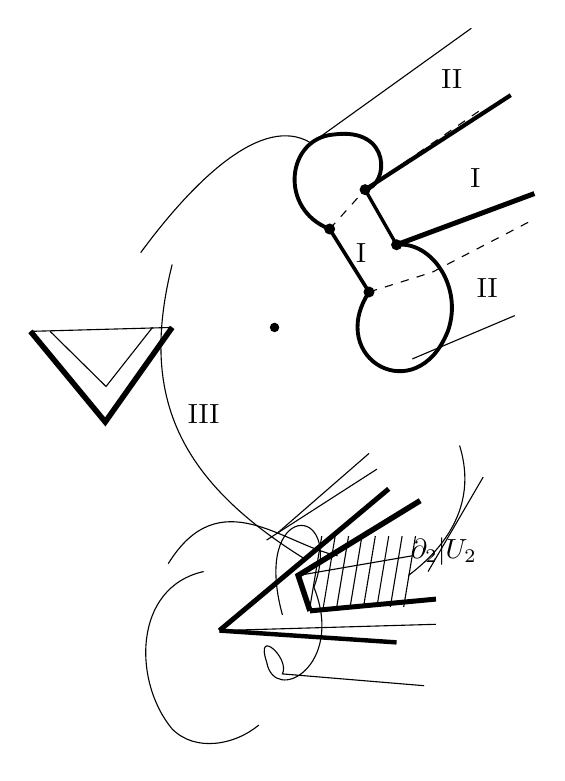
\begin{tikzpicture}[x=1cm,y=1cm]
\draw[line width=1.4pt] (3.8,4.45)..controls(3.15,4.7)and(3.25,5.6)..(3.85,5.65)..controls(4.6,5.75)and(4.55,5)..(4.25,4.95);
\draw[line width=1.3pt] (3.8,4.45)--(4.3,3.65);\draw[line width=1.2pt] (4.25,4.95)--(4.65,4.25);
\draw[line width=1.4pt] (4.3,3.65)..controls(3.75,2.8)and(4.9,2.15)..(5.3,3.15)..controls(5.5,3.7)and(5.1,4.3)..(4.65,4.25);
\draw (3.65,5.6)--(5.6,7);\draw[line width=1.5pt] (4.25,4.95)--(6.1,6.15);\draw[line width=1.8pt] (4.65,4.25)--(6.4,4.9);\draw (4.85,2.8)--(6.15,3.35);
\draw[dashed] (3.8,4.45)--(4.25,4.95)--(5.7,5.95);\draw[dashed] (4.3,3.65)--(5.1,3.9)--(6.35,4.55);
\foreach \p in {(3.8,4.45),(4.25,4.95),(4.3,3.65),(4.65,4.25)}{\fill \p circle(.07);}
\node at (5.35,6.35) {$\mathrm{II}$};\node at (5.65,5.1) {$\mathrm I$};\node at (4.2,4.15) {$\mathrm I$};\node at (5.8,3.7) {$\mathrm{II}$};
\fill (3.1,3.2) circle(.06);
\draw (1.4,4.15)..controls(2.1,5.1)and(2.95,5.9)..(3.55,5.55);
\draw (0,3.15)--(1.8,3.2);\draw[line width=2pt] (0,3.15)--(.95,2)--(1.8,3.2);\draw (.25,3.15)--(.96,2.45)--(1.55,3.2);
\draw (1.8,4)..controls(1.4,2.4)and(1.8,1.3)..(3.5,.25);\node at (2.2,2.1) {$\mathrm{III}$};
\draw (2.2,.1)..controls(1.3,-.1)and(1.3,-1.3)..(1.8,-1.9)..controls(2.1,-2.2)and(2.6,-2.1)..(2.9,-1.85);
\draw (1.75,.2)..controls(2.4,1.25)and(3.2,.45)..(3.9,.3);
\draw[line width=1.8pt] (2.4,-.65)--(4.55,1.15);\draw[line width=1.6pt] (2.4,-.65)--(4.65,-.8);
\draw[line width=2pt] (3.55,-.4)--(3.4,.05)--(4.95,1);\draw[line width=1.8pt] (3.55,-.4)--(5.15,-.25);
\draw (2.4,-.65)--(5.15,-.57);\draw (3.4,.05)--(4.85,.3);\draw (3,.5)--(4.4,1.4);\draw (3.15,.6)--(4.3,1.6);
\foreach \x in {3.55,3.72,...,4.75}{\draw (\x,-.35)--(\x+.15,.55);}
\draw (3.2,-.45)..controls(2.8,1)and(4,1)..(3.6,-.1)..controls(4,-1.1)and(3.1,-1.6)..(3,-1.05)..controls(2.85,-.6)and(3.3,-1)..(3.2,-1.2)--(5,-1.35);
\draw (4.8,.05)..controls(5.2,.35)and(5.7,.9)..(5.45,1.7);\draw (5.05,.1)--(5.75,1.3);
\node at (5.25,.35) {$\deleted{\unsure{\partial_2|U_2}}$};
\end{tikzpicture}}
% crop-candidate: scan 45

\figure{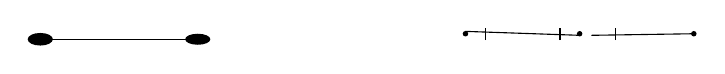
\begin{tikzpicture}[x=1cm,y=1cm]
\draw (0,0)--(2,0);\fill (0,0) ellipse(.16 and .08);\fill (2,0) ellipse(.16 and .07);
\draw (5.4,.1)--(6.85,.05);\draw (7,.05)--(8.3,.07);\foreach \x in {5.65,6.6,7.3}{\draw (\x,-.01)--(\x,.14);}\foreach \x in {5.4,6.85,8.3}{\fill (\x,.07) circle(.035);}
\end{tikzpicture}}

\figure{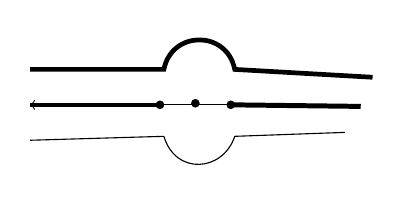
\begin{tikzpicture}[x=1cm,y=1cm]
\draw[line width=1.7pt] (0,.45)--(1.7,.45)..controls(1.8,.95)and(2.5,.95)..(2.6,.45)--(4.35,.35);
\draw[line width=1.3pt] (0,0)--(1.65,0);\draw (1.65,0)--(2.55,0);\draw[line width=1.8pt] (2.55,0)--(4.2,-.02);
\draw[<-] (0,0)--(.5,0);
\draw (0,-.45)--(1.7,-.4)..controls(1.85,-.9)and(2.45,-.85)..(2.6,-.4)--(4,-.35);
\foreach \p in {(1.65,0),(2.1,.02),(2.55,0)}{\fill \p circle(.055);}
\end{tikzpicture}}

\figure{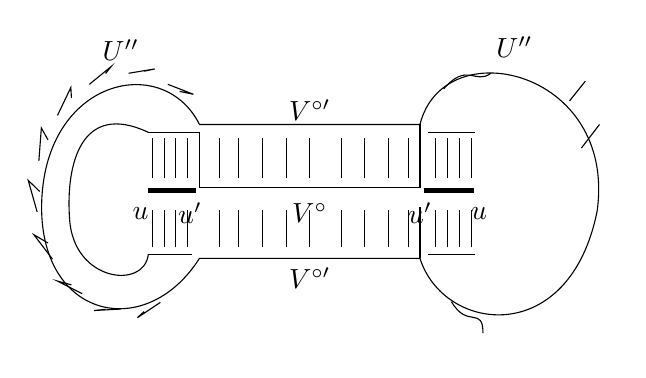
\begin{tikzpicture}[x=1cm,y=1cm]
\draw (0,1)..controls(-.45,1.9)and(-1.9,1.6)..(-2,.1)..controls(-2.1,-1.45)and(-.7,-1.8)..(0,-.7)--(2.8,-.7)..controls(3.1,-1.65)and(4.7,-1.85)..(5.05,-.1)..controls(5.3,1.7)and(3.1,2.2)..(2.8,1)--(0,1);
\draw (-.65,.9)..controls(-1.5,1.3)and(-1.7,.5)..(-1.65,-.2)..controls(-1.6,-1)and(-.7,-1.1)..(-.65,-.65);
\draw (-.65,.9)--(0,.9)--(0,.2)--(2.8,.2)--(2.8,1);\draw (-.65,-.65)--(-.1,-.65);\draw (2.8,-.7)--(2.8,-.05);
\draw[line width=1.8pt] (-.65,.16)--(-.05,.16);\draw[line width=1.8pt] (2.85,.16)--(3.48,.16);
\draw (2.9,.9)--(3.5,.9);\draw (2.9,-.65)--(3.5,-.65);
\foreach \x in {-.6,-.45,-.3,-.15,.25,.5,.8,1.1,1.4,1.8,2.1,2.4,2.65,3,3.15,3.3,3.45}{\draw (\x,.32)--(\x,.83);\draw (\x,-.56)--(\x,-.08);}
\foreach \a in {55,80,...,290}{\draw ({-.9+1.13*cos(\a)},{.15+1.55*sin(\a)})--({-.9+1.28*cos(\a-5)},{.15+1.61*sin(\a-5)})--({-.9+1.18*cos(\a+10)},{.15+1.5*sin(\a+10)});}
\draw (3.1,1.45)..controls(3.4,1.8)and(3.5,1.5)..(3.7,1.65);\draw (4.7,1.3)--(4.9,1.55);\draw (4.85,.7)--(5.08,1);\draw (3.2,-1.25)..controls(3.4,-1.6)and(3.6,-1.3)..(3.6,-1.65);
\node at (-1,1.95) {$U''$};\node at (4,1.98) {$U''$};\node at (1.4,1.18) {$V^{\circ\prime}$};\node at (1.4,-.95) {$V^{\circ\prime}$};\node at (1.4,-.12) {$V^\circ$};
\node at (-.75,-.13) {$u$};\node at (-.12,-.13) {$u'$};\node at (2.8,-.13) {$u'$};\node at (3.55,-.13) {$u$};
\end{tikzpicture}}

\figure{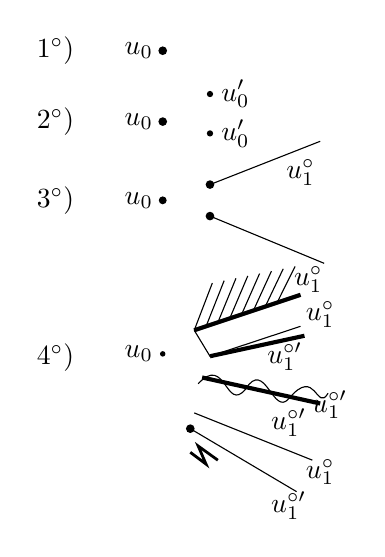
\begin{tikzpicture}[x=1cm,y=1cm]
\node[anchor=east] at (-1,8.8) {$1^\circ)$};\node[left] at (0,8.8) {$u_0$};\fill (0,8.8) circle(.055);
\node[anchor=east] at (-1,7.9) {$2^\circ)$};\node[left] at (0,7.9) {$u_0$};\fill (0,7.9) circle(.055);
\fill (.6,8.25) circle(.04);\node[right] at (.62,8.25) {$u'_0$};\fill (.6,7.75) circle(.04);\node[right] at (.62,7.75) {$u'_0$};
\node[anchor=east] at (-1,6.9) {$3^\circ)$};\node[left] at (0,6.9) {$u_0$};\fill (0,6.9) circle(.05);
\draw (.6,7.1)--(2,7.65);\draw (.6,6.7)--(2.05,6.1);\fill (.6,7.1) circle(.055);\fill (.6,6.7) circle(.055);\node at (1.75,7.25) {$u_1^\circ$};\node at (1.85,5.9) {$u_1^\circ$};
\node[anchor=east] at (-1,4.9) {$4^\circ)$};\node[left] at (0,4.95) {$u_0$};\fill (0,4.95) circle(.035);
\draw[line width=1.5pt] (.4,5.25)--(1.75,5.7);\draw (.4,5.25)--(.6,4.92)--(1.75,5.3);\draw[line width=1.5pt] (.6,4.92)--(1.8,5.18);
\foreach \x in {.4,.55,...,1.6}{\draw (\x,{5.25+(\x-.4)*.33})--({\x+.23},{5.85+(\x-.4)*.2});}
\node at (2,5.45) {$u_1^\circ$};\node at (1.55,4.92) {$u_1^{\circ\prime}$};
\draw[line width=1.5pt] (.5,4.65)--(2,4.32);\draw (.45,4.57)..controls(.8,4.95)and(.8,4.2)..(1.05,4.5)..controls(1.3,4.9)and(1.4,4.15)..(1.6,4.38)..controls(1.95,4.8)and(1.95,4.2)..(2.1,4.45);
\node at (2.12,4.3) {$\deleted{\unsure{u_1^{\circ\prime}}}$};
\draw (.4,4.2)--(1.9,3.6);\draw (.35,4.0)--(1.7,3.2);\fill (.35,4) circle(.055);\draw[line width=1pt] (.35,3.7)--(.55,3.55)--(.45,3.78)--(.7,3.6);
\node at (1.6,4.08) {$u_1^{\circ\prime}$};\node at (2,3.45) {$u_1^\circ$};\node at (1.6,3.02) {$u_1^{\circ\prime}$};
\end{tikzpicture}}

\figure{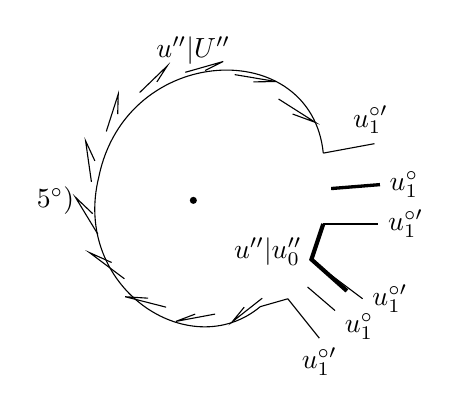
\begin{tikzpicture}[x=1cm,y=1cm]
\node at (-2.4,1) {$5^\circ)$};\fill (-.65,1) circle(.045);
\draw (1,1.6)..controls(.85,3.1)and(-1.5,3)..(-1.85,1.3)..controls(-2.2,-.1)and(-.7,-1.1)..(.2,-.35)--(.55,-.25);
\draw (1,1.6)--(1.65,1.72);\draw[line width=1.2pt] (1.1,1.15)--(1.72,1.2);\draw (1,.7)--(1.7,.7);\draw[line width=1.5pt] (1,.7)--(.85,.25)--(1.3,-.15);
\draw (.55,-.25)--(.95,-.75);\draw (.8,-.1)--(1.15,-.4);\draw (1.1,.05)--(1.5,-.25);
\foreach \a in {40,65,...,290}{\draw ({-.5+1.45*cos(\a)},{1.1+1.55*sin(\a)})--({-.5+1.65*cos(\a-8)},{1.1+1.68*sin(\a-8)})--({-.5+1.45*cos(\a+10)},{1.1+1.55*sin(\a+10)});}
\node at (-.65,2.9) {$\unsure{u''|U''}$};\node[above] at (1.6,1.72) {$u_1^{\circ\prime}$};\node[right] at (1.72,1.2) {$u_1^\circ$};\node[right] at (1.7,.7) {$u_1^{\circ\prime}$};\node[left] at (.85,.35) {$\unsure{u''|u_0''}$};
\node[right] at (1.5,-.25) {$u_1^{\circ\prime}$};\node[right] at (1.15,-.6) {$u_1^\circ$};\node[below] at (.95,-.75) {$u_1^{\circ\prime}$};
\end{tikzpicture}}

\figure{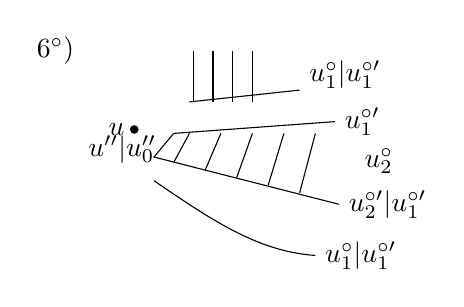
\begin{tikzpicture}[x=1cm,y=1cm]
\node at (-1.8,1.3) {$6^\circ)$};\node[left] at (-.8,.3) {$u$};\fill (-.8,.3) circle(.055);
\draw (-.1,.65)--(1.3,.8);\foreach \x in {-.05,.2,.45,.7}{\draw (\x,.65)--(\x,1.3);}\node[right] at (1.3,1) {$\unsure{u_1^\circ|u_1^{\circ\prime}}$};
\draw (-.3,.25)--(1.75,.4);\draw (-.3,.25)--(-.55,-.05)--(1.8,-.65);\foreach \x in {-.3,.1,.5,.9,1.3}{\draw (\x,{-.12-(\x+.3)*.24})--({\x+.2},.25);}
\draw (-.55,-.35)..controls(.25,-.9)and(.8,-1.25)..(1.5,-1.3);
\node[right] at (1.75,.4) {$u_1^{\circ\prime}$};\node[right] at (2,-.1) {$u_2^\circ$};\node[right] at (1.8,-.65) {$\unsure{u_2^{\circ\prime}|u_1^{\circ\prime}}$};\node[right] at (1.5,-1.3) {$\unsure{u_1^\circ|u_1^{\circ\prime}}$};\node[left] at (-.4,.05) {$\unsure{u''|u_0''}$};
\end{tikzpicture}}
\mspage{46}

\scanpage{46}
$\unsure{\Phi D|\Phi B}$\qquad variétés à bord fibrées sur v. à b. à fibres \unsure{id.|idem}

\figure{\begin{tikzpicture}[x=.5cm,y=.5cm]
\draw[gray!40] (3,18.8)..controls(3.4,18.7)and(3.7,18.8)..(4,18.9);
\draw[gray!35] (13.5,14.2)..controls(12.9,14.7)and(12.9,13.5)..(13.5,13.6)--(16.2,13.6)..controls(16.9,13.1)and(17,14.6)..(16.2,14.3)--(13.5,14.2);
\draw[gray!35] (13.4,13.95)--(16.5,13.9);\foreach \p in {(13.5,14.2),(13.5,13.6),(13.3,13.95),(16.2,14.3),(16.2,13.6),(16.5,13.9)}{\fill[gray!80] \p circle(.035);}
\draw[gray!30] (13.5,12.2)..controls(12.4,12.8)and(11.9,10.6)..(13.2,10.7)--(15.9,10.8)..controls(16.9,10.1)and(17.4,12.5)..(16.1,12.5)--(13.5,12.2);
\draw[gray!30] (13.35,11.85)--(16.1,11.85);\draw[gray!30] (13.35,11.2)--(16.1,11.15);\draw[gray!30] (13.2,11.5)--(14.8,9.75)--(16.6,11.5);
\foreach \p in {(13.5,12.2),(13.2,11.5),(13.35,11.2),(16.1,12.2),(16.6,11.5),(14.8,9.75)}{\fill[gray!65] \p circle(.04);}
\draw[gray!35] (0,12.1)--(2.5,10.4);\draw[gray!30] (0,10.4)--(2.2,9.8);\draw[gray!35] (2.5,10.4)..controls(2.7,11.6)and(4,11.2)..(3.45,10.15)--(2.85,9.25)..controls(3.4,8.25)and(2.15,8.1)..(1.7,8.7);
\draw[gray!55] (2.5,10.4)--(2.2,9.8);\foreach \p in {(2.5,10.4),(2.2,9.8),(3.45,10.15)}{\fill[gray!80] \p circle(.045);}
\draw[gray!55] (6.25,8.5)--(7.05,7.3)--(8.3,8.45);\draw[gray!25] (6.55,8.5)--(7.05,7.65)--(8.1,8.45);\fill (7.05,7.3) circle(.045);
\fill[gray!50] (16,8.9)--(16.35,9.5)--(16.9,9.3)--(17.6,8.35)--(17.1,7.95)--cycle;
\draw[gray!25] (2.8,6.9)--(5.05,5.65)--(2.9,5.75);\draw[gray!40] (3.8,6.6)--(4.4,6.05)--(4.2,5.7);\draw[gray!20] (2.8,6.65)--(5,5.45)--(2.7,5.4);\draw[gray!80] (4.18,6.02)--(4.35,5.87)--(4.22,5.65);
\draw[gray!20] (9.05,5.5)--(10.5,5.4)--(11.1,5.45);\fill[gray!70] (14.8,5.35) circle(.035);\fill[gray!80] (16.55,5.3) circle(.055);
\draw[gray!50] (8.3,3.9)--(9.5,3.9)..controls(9.7,4.4)and(10.2,4.4)..(10.35,3.9)--(11.7,3.95);
\draw[gray!60] (8.1,3.5)--(9.5,3.5);\draw[gray!55] (10.4,3.48)--(11.15,3.43);\draw[gray!30] (8.2,3.15)--(9.5,3.15)..controls(9.7,2.6)and(10.2,2.65)..(10.35,3.15)--(11.1,3.1);
\draw[gray!15] (13.2,2.35)..controls(12.8,3.1)and(11.9,2.55)..(12,1.1)..controls(12.3,.4)and(13,.5)..(13.2,1.0)--(16,1)..controls(16.5,.1)and(17.8,.6)..(17.4,2.5)..controls(17.1,3.4)and(16.3,3)..(16,2.35)--(13.2,2.35);
\draw[gray!20] (13.2,1.7)--(16.2,1.7);\fill[gray!55] (12.9,1.7) circle(.025);\fill[gray!55] (16.45,1.67) circle(.03);
\fill[gray!75] (4.55,3.0) circle(.025);\fill[gray!70] (4.1,2.1) circle(.025);
\draw[gray!20] (2.65,1.3)--(4.7,1.95);\draw[gray!20] (2.7,1.0)--(4.65,.2);\draw[gray!45] (3.15,.5)--(4.3,.1);
\draw[gray!18] (2.8,.15)--(4.3,-.5);\draw[gray!40] (3.05,-.4)--(4,-.75);\draw[gray!35] (2.95,-1.05)--(3.7,-.82);\draw[gray!15] (2.8,-1.1)--(4.4,-1.85);\draw[gray!15] (2.9,-2.2)--(4.25,-1.35);
\draw[gray!15] (3.3,-3.6)--(4.3,-3.8)--(3.6,-4.4)--(4.5,-4.9);\draw[gray!20] (3.45,-4.4)--(3.85,-5.1);\draw[gray!18] (3.65,-5.5)--(5.3,-5.7)--(3.5,-6.2);\draw[gray!18] (3.5,-6.35)--(5.15,-5.85);\draw[gray!25] (4,-6.75)--(5.1,-6.3);
\foreach \p in {(3.9,-3.1),(4.2,-3.4),(4.75,-3.85),(3.9,-4.9),(5.5,-5.3)}{\fill[gray!50] \p circle(.025);}
\end{tikzpicture}}
\mspage{47}

\scanpage{47}
\diagram{\begin{tikzcd}
\partial_j V_i^\circ \arrow[r] & V_j^\circ
\end{tikzcd}}

\diagram{\begin{tikzcd}[column sep=small,row sep=large]
\partial(\partial_j V_i^\circ)=\displaystyle\bigcup_{k\in\Phi_j} & \underbracket{\partial_j V_i^\circ\mid\partial_k V_j^\circ}_{\vphantom{V}}\arrow[d] & \cup & \underbracket{\partial^{\unsure{\mathrm{pr}|\mathrm{rel}}}\partial_j V_i^\circ}_{\vphantom{V}}\arrow[d]\\
&V_k^\circ&&V_j^\circ
\end{tikzcd}}

\diagram{\begin{tikzcd}[column sep=small,row sep=large]
\underset{n_i}{V_i^\circ}\arrow[r,-{Hooks[harpoon]}]&
\underset{n_i-1}{\partial V_i^\circ}\arrow[r,-{Hooks[harpoon]}]&
\underset{n_i-1}{V_{ij}^\circ}\arrow[r,-{Hooks[harpoon]}]\arrow[d,"{\deleted{\unsure{n_i}}}"']\arrow[drr,phantom,"\times"]&
\partial V_{ij}^\circ\arrow[r,-{Hooks[harpoon]}]\arrow[r,dash,start anchor=north,end anchor=north,to path={(\tikztostart)--++(0,.25)-|(\tikztotarget)\tikztonodes}]&
\underset{n_i-2}{V_{ij}^\circ\mid\partial V_j^\circ}\arrow[r,-{Hooks[harpoon]}]\arrow[d]\arrow[dr,phantom,"\times"]&
\underset{n_{\unsure{j|i}}-2}{V_{ijk}^\circ}\arrow[d]\arrow[drr,phantom,"\times"]&&
V_{ijk}^\circ\mid\partial V_k^\circ\arrow[ll]\arrow[d]\arrow[dr,phantom,"\times"]&
\underset{n_i-3}{V_{ijk\ell}^\circ}\arrow[l]\arrow[d]\\
&&\underset{n_j}{V_j^\circ}\arrow[rr,-{Hooks[harpoon]}]&&
\underset{n_j-1}{\partial V_j^\circ}\arrow[r,-{Hooks[harpoon]}]&
\underset{n_j-1}{V_{jk}^\circ}\arrow[r,-{Hooks[harpoon]}]\arrow[d]\arrow[drr,phantom,"\times"]&
\underset{n_j-2}{\deleted{\partial V_{jk}^\circ}}&
V_{jk}^\circ\mid\partial V_k^\circ\arrow[l]\arrow[d]\arrow[dr,phantom,"\times"]&
V_{jk\ell}^\circ\arrow[l]\arrow[d]\\
&&&&&V_k^\circ&&\partial V_k^\circ\deleted{{}_{\unsure{\ell}}}\arrow[ll]&V_{k\ell}^\circ\arrow[l]\arrow[d]\\
&&&&&&&&V_\ell^\circ
\end{tikzcd}}

\diagram{\begin{tikzcd}[column sep=small,row sep=large]
V_i^\circ&V_{ij}^\circ\arrow[l]\arrow[d]\arrow[dr,phantom,"\times"]&V_{ijk}^\circ\arrow[l]\arrow[d]\arrow[dr,phantom,"\times"]&V_{ijk\ell}^\circ\arrow[l]\arrow[d]\arrow[dr,phantom,"\times"]&\cdots\arrow[l]\arrow[dr,phantom,"\times"]&V_{ijk\ell\cdots p}^\circ\arrow[l]\arrow[d]\\
&V_j^\circ&V_{jk}^\circ\arrow[l]\arrow[d]\arrow[dr,phantom,"\times"]&V_{jk\ell}^\circ\arrow[l]\arrow[d]\arrow[dr,phantom,"\times"]&\cdots\arrow[l]\arrow[dr,phantom,"\times"]&V_{jk\ell\cdots p}^\circ\arrow[l]\arrow[d]\\
&&V_k^\circ&V_{k\ell}^\circ\arrow[l]\arrow[d]\arrow[dr,phantom,"\times"]&\cdots\arrow[l]\arrow[dr,phantom,"\times"]&V_{k\ell\cdots p}\arrow[l]\arrow[d]\\
&&&V_\ell^\circ&\cdots\arrow[l]\arrow[dr,phantom,"\times"]&V_{\ell\cdots p}\arrow[l]\arrow[d]\\
&&&&\cdots&\substack{\cdots\cdot\cdot\\[-.5ex]\vdots\\[-.5ex]\cdots\cdot\cdot}\arrow[d]\\
&&&&&V_p^\circ
\end{tikzcd}}
\mspage{48}

\scanpage{48}
\uline{Équisingularité}

\uline{\unsure{Cellules}}

\mspage{49}
